% -*- TeX:UTF-8 -*-
%%
%% KAIST 학위논문양식 LaTeX용 (ver 0.5) 예시
%%
%% @version 0.4
%% @author  채승병 Chae,Seungbyung (mailto:chess@kaist.ac.kr)
%% @date    2004. 11. 12.
%%
%% @requirement
%% teTeX, fpTeX, teTeX 등의 LaTeX2e 배포판
%% + 은광희 님의 HLaTeX 0.991 이상 버젼 또는 홍석호 님의 HPACK 1.0
%% : 설치에 대한 자세한 정보는 http://www.ktug.or.kr을 참조바랍니다.
%%
%% @note
%% 기존에 널리 쓰여오던 차재춘 님의 학위논문양식 클래스 파일의 형식을
%% 따르지 않고 전면적으로 다시 작성하였습니다. 논문 정보 입력부분에서
%% 과거 양식과 다른 부분이 많으니 아래 예시에 맞춰 바꿔주십시오.
%%
%%
%% @acknowledgement
%% 본 예시 논문은 물리학과 박사과정 김용현 님의 호의로 제공되었습니다.
%%
%% -------------------------------------------------------------------
%% @information
%% 이 예제 파일은 hangul-ucs를 사용합니다. UTF-8 입력 인코딩으로
%% 작성되었습니다. hlatex의 hfont는 이용하지 않습니다. --2006/02/11
%% 본 템플릿은 전산학부 김민혁 교수에의해서 버그 수정되었습니다. -- 2016/11/25

% @class kaist.cls
% @options [default: doctor, korean, final]
% - doctor: 박사과정 | master : 석사과정
% - korean: 한글논문 | english: 영문논문
% - final : 최종판   | draft  : 시험판
% - pdfdoc : 선택하지 않으면 북마크와 colorlink를 만들지 않습니다.


\documentclass[master,english,final]{kaist-ucs}
% If you want make pdf document (include bookmark, colorlink)
%\documentclass[doctor,english,final,pdfdoc]{kaist-ucs}

% kaist.cls 에서는 기본으로 dhucs, ifpdf, graphicx 패키지가 로드됩니다.
% 추가로 필요한 패키지가 있다면 주석을 풀고 적어넣으십시오,
%\usepackage{...}
\usepackage[T1]{fontenc}
\usepackage{lmodern}
\usepackage{parskip}        % Package to tweak paragraph skipping (instead of indents a small skip is added after every paragraph)
\usepackage{titlesec}
%\usepackage{tikz}           % Package for drawing
\usepackage{pgfplots}       % Package for creating graphs and charts
\usepackage{xcolor}         % Package for defining DTU colours to be used
% Colours!
\newcommand{\targetcolourmodel}{cmyk} % rgb for a digital version, cmyk for a printed version. Only use lowercase
\selectcolormodel{\targetcolourmodel}

% Define colours from https://www.designguide.dtu.dk/
\definecolor{dtured}    {rgb/cmyk}{0.6,0,0 / 0,0.91,0.72,0.23}
\definecolor{blue}      {rgb/cmyk}{0.1843,0.2431,0.9176 / 0.88,0.76,0,0}
\definecolor{brightgreen}{rgb/cmyk}{0.1216,0.8157,0.5098 / 0.69,0,0.66,0}
\definecolor{navyblue}  {rgb/cmyk}{0.0118,0.0588,0.3098 / 1,0.9,0,0.6}
\definecolor{yellow}    {rgb/cmyk}{0.9647,0.8157,0.3019 / 0.05,0.17,0.82,0}
\definecolor{orange}    {rgb/cmyk}{0.9882,0.4627,0.2039 / 0,0.65,0.86,0}
\definecolor{pink}      {rgb/cmyk}{0.9686,0.7333,0.6941 / 0,0.35,0.26,0}
\definecolor{grey}      {rgb/cmyk}{0.8549,0.8549,0.8549 / 0,0,0,0.2}
\definecolor{red}       {rgb/cmyk}{0.9098,0.2471,0.2824 / 0,0.86,0.65,0}
\definecolor{green}     {rgb/cmyk}{0,0.5333,0.2078 / 0.89,0.05,1,0.17}
\definecolor{purple}    {rgb/cmyk}{0.4745,0.1373,0.5569 / 0.67,0.96,0,0}
\definecolor{kaistblue} {rgb/cmyk}{0,0.65,0.145 / 1,0.75,0,0.1}
\definecolor{LightGray}{gray}{0.9}
\selectcolormodel{natural}
\usepackage{ninecolors}
\selectcolormodel{rgb}
\usepackage{amsmath}        % For aligning equations among other
\usepackage{mathtools}		% Extensible symbols, brackets, arrows, etc
\usepackage{xfrac}			% More modern than nicefrac
\usepackage{listings}       % Package for inserting code, (before cleveref)
\usepackage[chapter]{minted}
%\setminted{autogobble,linenos=true,breaklines,labelposition=all}
\usepackage[most, minted]{tcolorbox}
%\usepackage[most]{tcolorbox}
%\tcbuselibrary{listings, breakable, skins}
\PassOptionsToPackage{hyphens}{url} % Ability to line break urls at hyphens
\usepackage{cleveref}       % improved cross referencing
\usepackage{textcomp}       % \textdegree = °C and other useful symbols
\usepackage{caption}        % better captions
\usepackage{subcaption}     % for subfigures
\usepackage[autostyle=true]{csquotes}       % For biblatex with babel
\usepackage[backend=biber,style=ieee,abbreviate=true,dateabbrev=false,alldates=long,sorting=ynt,dashed=false,block=space,mincitenames=1,maxcitenames=1,maxbibnames=9,backref=false]{biblatex} % Package for bibliography (citing)
\bibliography{bib_bibertool.bib}

% Tables
\usepackage{float}          % floating figures in correct places
\usepackage{adjustbox}				% Adjust table widths (?)
\usepackage{nth}			% 1st, 2nd, etc
\usepackage{tabularray}		% latex3 tables
\UseTblrLibrary{booktabs,siunitx,varwidth}

% Extras
\usepackage[automake=immediate,toc, % Abbreviations and glossary lists
abbreviations,
postdot,
hyperfirst=true,
nopostdot=true,
nonumberlist=true,
nowarn,
]{glossaries-extra}
\usepackage{glossary-longextra} % Long booktabs table style
\usepackage[numbib]{tocbibind} % Lists of... in toc
%\usepackage{tocloft}		% Customising toc
%\usepackage{calc}           % Adds ability for latex to calculate (3pt+2pt)
\usepackage{blindtext}
\usepackage{graphicx}
\graphicspath{{Figures/}} %Setting the graphicspath
\usepackage{svg}
\usepackage[colorinlistoftodos]{todonotes} % Margin coloured todonotes
\usepackage{pdflscape}
% Drawing
\usepackage{tikz}					% Create graphics
\usetikzlibrary{arrows.meta,chains,backgrounds,positioning,fit,petri,automata,quotes}
\usepackage{xstring}				% For manipulating strings. Required by CircuiTikZ
\usepackage[american,arrowmos,nooldvoltagedirection]{circuitikz}	% Create circuit graphics (using TikZ)

\usepackage[verbose=silent,protrusion=true,expansion=true,final,babel]{microtype} % Better text appearance
\usepackage{hyphenat}			% Prevent hyphenation by \nohyphens{text}
\usepackage{pgfgantt}

% mathtools configuration
% Swap the definition of \abs* and \norm*, so that \abs
% and \norm resizes the size of the brackets, and the
% starred version does not.

\DeclarePairedDelimiter\abs{\lvert}{\rvert}%
\DeclarePairedDelimiter\norm{\lVert}{\rVert}%

\makeatletter
\let\oldabs\abs
\def\abs{\@ifstar{\oldabs}{\oldabs*}}
%
\let\oldnorm\norm
\def\norm{\@ifstar{\oldnorm}{\oldnorm*}}
\makeatother

\newtcblisting{mintedc}{%
	listing engine=minted,
	minted language=c,
	listing only,
	breakable,
	enhanced,
	minted options = {
		linenos,
		breaklines=true,
		breakbefore=.,
		fontsize=\footnotesize,
		numbersep=2mm
	},
	overlay={%
		\begin{tcbclipinterior}
			\fill[gray!25] (frame.south west) rectangle ([xshift=4mm]frame.north west);
		\end{tcbclipinterior}
	}
}

\newtcblisting{mintedmatlab}{%
	listing engine=minted,
	minted language=matlab,
	listing only,
	breakable,
	enhanced,
	minted options = {
		linenos,
		breaklines=true,
		breakbefore=.,
		fontsize=\footnotesize,
		numbersep=2mm
	},
	overlay={%
		\begin{tcbclipinterior}
			\fill[gray!25] (frame.south west) rectangle ([xshift=4mm]frame.north west);
		\end{tcbclipinterior}
	}
}

\newtcblisting{mintedvhdl}{%
	listing engine=minted,
	minted language=vhdl,
	listing only,
	%	breakable,
	%	enhanced,
	minted options = {
		linenos,
		breaklines=true,
		%		breakbefore=.,
		fontsize=\footnotesize,
		numbersep=2mm
	},
	overlay={%
		\begin{tcbclipinterior}
			\fill[gray!25] (frame.south west) rectangle ([xshift=4mm]frame.north west);
		\end{tcbclipinterior}
	}
}

\newtcblisting{mintedpython}{%
	listing engine=minted,
	minted language=python,
	listing only,
	%	breakable,
	%	enhanced,
	minted options = {
		linenos,
		breaklines=true,
		%		breakbefore=.,
		fontsize=\footnotesize,
		numbersep=2mm
	},
	overlay={%
		\begin{tcbclipinterior}
			\fill[gray!25] (frame.south west) rectangle ([xshift=4mm]frame.north west);
		\end{tcbclipinterior}
	}
}

\BeforeBeginEnvironment{minted}
{ \begin{tcolorbox}[breakable, enhanced] }

	\AfterEndEnvironment{minted}
	{ \end{tcolorbox} }


\newcommand{\documenttype}{Master Thesis}
\newcommand{\thesistitle}{Portable Ultrasound System for Blood Velocity Estimation}
\newcommand{\thesissubtitle}{Project Report}

\newcommand{\thesisauthor}{Jeppe Hinrichs} % Your name :) 
\newcommand{\studentnumber}{s163555}
\newcommand{\thedate}{March, 2023} % For example "June, 2019"

\newcommand{\dtudepartment}{DTU Electrical Engineering}
\newcommand{\dtudepartmentdescriber}{Department of Electrical Engineering}
\newcommand{\dtuorg}{Technical University of Denmark}
\newcommand{\dtuaddressI}{Ørsteds Plads, Building 348}
\newcommand{\dtuaddressII}{2800 Kgs. Lyngby}
\newcommand{\dtudepartmentwebsite}{www.elektro.dtu.dk}

\newcommand{\kaistdepartment}{KAIST EE}
\newcommand{\kaistdepartmentdescriber}{School of Electrical Engineering}
\newcommand{\kaistorg}{Korea Advanced Institute of Science and Technology}
\newcommand{\kaistaddressI}{291 Daehak-ro, Yuseong-gu}
\newcommand{\kaistaddressII}{34141 Daejeon}
\newcommand{\kaistdepartmentwebsite}{www.ee.kaist.ac.kr}

\newcommand{\projectstartdate}{\formatdate{1}{9}{2022}}
\newcommand{\projectenddate}{\formatdate{1}{2}{2023}}
\newcommand{\projectcredits}{30 ECTS / 9 credits}
\newcommand{\degreename}{Electrical Engineering}
\newcommand{\degreetype}{Master of Science}
\makeglossaries
\setabbreviationstyle{long-short-sc}

\newglossaryentry{high}{
	name=HIGH,
	description={Logic high voltage level},
    category={glosscat}
}

\newglossaryentry{low}{
	name=LOW,
	description={Logic low voltage level},
    category={glosscat}
}

\newglossaryentry{spice}{
	name=SPICE,
	description={SPICE ("Simulation Program with Integrated Circuit Emphasis") is an open-source IC and board-level circuit simulator},
	category={glosscat}
}

\newglossaryentry{ltspice}{
	name=LTspice,
	description={A freeware \glsxtrshort{spice}-based circuit simulator from Linear Technology/Analog Devices},
    category={glosscat}
}

\newglossaryentry{csv}{
	name=CSV,
	description={A text file that uses a comma (,) to separate each table value},
	category={glosscat}
}

\newglossaryentry{rmc}{
	name=RMC,
	description={Root mean square, or quadratic mean value},
	category={glosscat}
}

\newglossaryentry{c}{
	name={C},
	description={General purpose computer programming language},
	category={glosscat}
}

\newglossaryentry{cpp}{
	name={C++},
	description={High-level general purpose programming language, derived from C},
	category={glosscat}
}

\newglossaryentry{rtos}{
	name={Real-time operating system},
	description={Operating systems with critically defined time constraints for real-time processing},
	category={glosscat}
}

\newglossaryentry{matlab}{
	name=MATLAB,
	description={Computing environment used for matrices, plotting and simulation interfacing},
	category={glosscat}
}

\newglossaryentry{adiabatic}{
	name=adiabatic,
	description={Any process that happens without heat gain or loss is considered adiabatic},
	category={glosscat}
}


\newabbreviation[category={acronymcat}]{ac}{AC}{Alternating Current}

\newabbreviation[category={acronymcat}]{dc}{DC}{Direct Current}

\newabbreviation[category={acronymcat}]{mcu}{MCU}{Microcontroller Unit}

\newabbreviation[category={acronymcat}]{gcd}{GCD}{Greatest Common Divisor}

\newabbreviation[category={acronymcat}]{lcm}{LCM}{Least Common Multiple}

\newabbreviation[category={acronymcat}]{aim}{AIM}{Astable Integrating Modulator}

\newabbreviation[category={acronymcat}]{bpf}{BPF}{Band-Pass Filter}

\newabbreviation[category={acronymcat}]{btl}{BTL}{Bridge-Tied Load}

\newabbreviation[category={acronymcat}]{emi}{EMI}{Electromagnetic Interference}

\newabbreviation[category={acronymcat}]{esr}{ESR}{Equivalent Series Resistance}

\newabbreviation[category={acronymcat}]{hpf}{HPF}{High-Pass Filter}

\newabbreviation[category={acronymcat}]{kcl}{KCL}{Kirchoff's Current Law}

\newabbreviation[category={acronymcat}]{kvl}{KVL}{Kirchoff's Voltage Law}

\newabbreviation[category={acronymcat}]{lqr}{LQR}{Linear Quadratic Regulator}

\newabbreviation[category={acronymcat}]{fet}{MOSFET}{Metal-Oxide-Semiconductor Field-Effect Transistor}

\newabbreviation[category={acronymcat}]{opamp}{OP-AMP}{Operational Amplifier}

\newabbreviation[category={acronymcat}]{pcm}{PCM}{Pulse Code Modulation}

\newabbreviation[category={acronymcat}]{pi}{PI}{Proportional-Integral Regulator}

\newabbreviation[category={acronymcat}]{pid}{PID}{Proportional-Integral-Derivative Regulator}

\newabbreviation[category={acronymcat}]{pwm}{PWM}{Pulse-Width Modulation}

\newabbreviation[category={acronymcat}]{rlc}{RLC}{Resistor-Inductor-Capacitor}

\newabbreviation[category={acronymcat}]{rms}{RMS}{Root-Mean-Square}

\newabbreviation[category={acronymcat}]{rvs}{RVS}{Reduced Voltage Switching}

\newabbreviation[category={acronymcat}]{smps}{SMPS}{Switched-Mode Power Supply}

\newabbreviation[category={acronymcat}]{snr}{SNR}{Signal-to-Noise Ratio}

\newabbreviation[category={acronymcat}]{mri}{MRI}{Magnetic Resonance Imaging}

\newabbreviation[category={acronymcat}]{1d}{1D}{One-Dimensional}

\newabbreviation[category={acronymcat}]{2d}{2D}{Two-Dimensional}

\newabbreviation[category={acronymcat}]{3d}{3D}{Three-Dimensional}

\newabbreviation[category={acronymcat}]{ca}{CA}{Carotid Artery}

\newabbreviation[category={acronymcat}]{cad}{CAD}{Computer Aided Design}

\newabbreviation[category={acronymcat}]{ct}{CT}{Computed Tomography}

\newabbreviation[category={acronymcat}]{dtu}{DTU}{Danmarks Tekniske Universitet (Technical University of Denmark)}

\newabbreviation[category={acronymcat}]{kaist}{KAIST}{Korea Advanced Institute of Science and Technology}

\newabbreviation[category={acronymcat}]{rx}{Rx}{Receive}

\newabbreviation[category={acronymcat}]{tx}{Tx}{Transmit}

\newabbreviation[category={acronymcat}]{mux}{Mux}{Multiplexer}

\newabbreviation[category={acronymcat}]{US}{us}{Ultrasound}

\newabbreviation[category={acronymcat}]{sdu}{SDU}{Spectral Doppler Ultrasound}

\newabbreviation[category={acronymcat}]{prf}{PRF}{Pulse Repetition Frequency}

\newabbreviation[category={acronymcat}]{rf}{RF}{Radio Frequency}

\newabbreviation[category={acronymcat}]{fft}{FFT}{Fast-Fourier Transform}

\newabbreviation[category={acronymcat}]{ft}{FT}{Fourier Transform}

\newabbreviation[category={acronymcat}]{lp}{LP}{Low-pass}

\newabbreviation[category={acronymcat}]{hp}{HP}{High-pass}

\newabbreviation[category={acronymcat}]{bp}{BP}{Band-pass}

\newabbreviation[category={acronymcat}]{adc}{ADC}{Analogue-to-Digital Converter}

\newabbreviation[category={acronymcat}]{dac}{dac}{Digital-to-Analogue Converter}

\newabbreviation[category={acronymcat}]{sh}{S/H}{Sample/Hold}

\newabbreviation[category={acronymcat}]{cw}{CW}{Continuous Wave}

\newabbreviation[category={acronymcat}]{pw}{PW}{Pulsed Wave}

\newabbreviation[category={acronymcat}]{fifo}{FIFO}{First-In First-Out}

\newabbreviation[category={acronymcat}]{fir}{FIR}{Finite Impulse Response}

\newabbreviation[category={acronymcat}]{dsp}{DSP}{Digital Signal Processor}

\newabbreviation[category={acronymcat}]{low-res}{low-res}{Low Resolution}


% @command title 논문 제목(title of thesis)
% @options [default: (none)]
% - korean: 한글제목(korean title) | english: 영문제목(english title)
\title[korean] {혈류 속도 예측을 위한 휴대용 초음파 시스템}
\title[english]{Portable ultrasound system for blood velocity estimation}

% @note 표지에 출력되는 제목을 강제로 줄바꿈하려면 \linebreak 을 삽입.
%       \\ 나 \newline 등을 사용하면 안됩니다. (아래는 예시)
%
%\title[korean]{탄소 나노튜브의 물리적 특성에 대한\linebreak 이론 연구}
%\title[english]{Theoretical study on physical properties of\linebreak
	%                carbon nanotubes}
%
% If you want to begin a new line in cover, use \linebreak .
% See examples above.
%


% @command author 저자 이름
% @param   family_name, given_name 성, 이름을 구분해서 입력
% @options [default: (none)]
% - korean: 한글이름 | chinese: 한문이름 | english: 영문이름
% 한문 이름이 없다면 빈 칸으로 두셔도 됩니다.
%
%
% If you are a foreigner , write your name in korean or your korean name.
% If you can't write native character, you can make the chinese blank empty
% Write as follow
% \author[korean]{family name in korean}{given name in korean}
% \author[chinese]{family name in your native language}{given name in your native language}
% \author[english]{family name in english}{given name in english}
%
\author[korean]{힌릭스}{예페}
\author[korean2]{힌릭스}{예페}   %이름을 붙여 써 주시기 바랍니다.
\author[chinese]{}{}
\author[english]{Hinrichs}{Jeppe}

% @command advisor 지도교수 이름 (복수가능)
% @usage   \advisor[options]{...한글이름...}{...영문이름...}{signed|nosign}
% @options [default: major]
% - major: 주 지도교수  | coopr: 공동 지도교수
\advisor[major]{이 현 주}{Hyunjoo Lee}{signed}
\advisor[major2]{}{Fafoutis Xenofon}{signed}    %한글 성과 한글 이름을 모두 붙여 써 주시기 바랍니다.
\advisorinfo{Professor of Electrical Engineering} %제출승인서에 들어가는 교수님 정보, advisor's information
%\advisor[coopr]{홍 길 동}{Gil-Dong Hong}{nosign}
%\advisor[coopr2]{홍길동}{Gil-Dong Hong}{nosign}    %한글 성과 한글 이름을 모두 붙여 써 주시기 바랍니다.
%
% 지도교수 한글이름은 입력하지 않아도 됩니다.
% You may not input advisor's korean name
% like this \advisor[major]{}{Chang, Kee Joo}{signed}
%


% @command department {학과이름}{학위종류} - 아래 규칙에 따라 코드를 입력
% @command department {department code}{degree field}
%
% department code
% 2. 석박사학위논문 작성 및 제출요령 4쪽 ~ 5쪽 참고
% 또는 kaist-ucs.cls 의 % @command department 참고

% science: 이학 | engineering: 공학 | business : 경영학
% 박사논문의 경우는 학위종류를 입력하지 않아도 됩니다.
% If you write Ph.D. dissertation, you cannot input degree field.
% The third parameter : a | b | c
% a: 소속된 학과만 쓰는 옵션 (학과에만 소속되어 있는 경우에는 무조건 a를 선택해야 함)
% b: 학과 아래의, 프로그램이나 학제전공에 소속되어 있을 경우에 학과와 프로그램을 함께 쓰는 옵션
% c: 학과 아래의, 프로그램이나 학제전공에 소속되어 있을 경우에 학과를 쓰지 않고 프로그램이나 학제전공의 이름만 쓰는 옵션
%
% a: it represents only the name of department. (if you aren't in the program under the department, must choose a)
% b: it represents the names of department and the program that is under the department (consider this when you are in the program not only department)
% c: it represents only the name of program that is under the department (consider this when you are in the program not only department)
\department{EE}{engineering}{a}

% @command referee 심사위원 (석사과정 3인, 박사과정 5인)
\referee[1]{이 현 주}
\referee[2]{Fafoutis Xenofon}
\referee[3]{제 민 규}
%\referee[4]{Zsurzsan Tiberiu Gabriel}
%\referee[5]{Micconi Laura}
% \referee[5] {Barack Obama}
% Of course english name is available

% @command approvaldate 지도교수논문승인일
% @param   year,month,day 연,월,일 순으로 입력
\approvaldate{2023}{6}{15}

% @command refereedate 심사위원논문심사일
% @param   year,month,day 연,월,일 순으로 입력
\refereedate{2023}{6}{15}

% @command gradyear 졸업년도
\gradyear{2023}

% 본문 시작
\makeglossaries

\begin{document}


	% 앞표지, 속표지, 학위논문 제출승인서, 학위논문 심사완료 검인서는
	% 클래스 옵션을 final로 지정해주면 자동으로 생성되며,
	% 반대로 옵션을 draft로 지정해주면 생성되지 않습니다.

	% 논문 서지, 초록, 핵심 낱말, 영문 초록, 영어 핵심 낱말 (Information of thesis, abstract in korean, keywords in korean, abstract in english, keywords in english)
	\thesisinfo
	%% Letters of abstract in korean must be less than 500 and words of abstract in english must be less than 300.
	%% Number of keywords must be less than 6.
	%% Don't write english letters in the abstract in korean.
	\begin{summary}
		초음파 이미징은 혈류 측정을 수행하는 중요한 방법이다. 이 보고서는 그러한 초음파 혈 류 측정 시스템의 설계, 구현과 분석을 담고 있다. 초음파 혈류 측정 시스템은 Xilinx Zynq	7000 SoC 라는 중앙 제어 시스템을 기반으로 자체 제작된 아날로그 프론트 엔드를 구현하	기 위한 다양한 초음파 펄스 및 타이밍 신호를 발생시킨다. 또한, 이 시스템은 직교 복조를 이용하여 복조된 도플러 주파수를 얻는다. 모듈 단위로 시스템을 테스트하였으나 시간 제 약으로 인해 전체를 테스트하지는 못하였다.
	\end{summary}

	\begin{Korkeyword}
		인지 무선 통신, 협력 통신, 중계, 전 이중, 동시 송수신
	\end{Korkeyword}


	\begin{abstract}
		For blood flow estimation, ultrasound imaging is an important tool. This project report outlines the design, implementation, and analysis of such ultrasound blood velocity estimator. The design is based off a central control system on a Xilinx Zynq 7000 SoC for generating ultrasound pulses and the various timing signals needed for operating the custom designed analogue front-end. The chosen design topology uses a pulsed-wave design with quadrature demodulation to obtain the Doppler frequency. The system was module tested, but was not fully end-to-end tested on a physiological simulator due to time constraints.
	\end{abstract}

	\begin{Engkeyword}
		Ultrasound, biomedical, imaging, blood velocity, velocity estimation, cvd, blood flow, RF, analogue electronics, VHDL, FPGA, embedded systems, pulser
	\end{Engkeyword}


	\addtocounter{pagemarker}{1}                 % 백색별지분을 고려
	\newpage



	% 목차 (Table of Contents) 생성
	\tableofcontents

	% 표목차 (List of Tables) 생성
	\listoftables

	% 그림목차 (List of Figures) 생성
	\listoffigures

	% 위의 세 종류의 목차는 한꺼번에 다음 명령으로 생성할 수도 있습니다.
	%\makecontents

	%% 이하의 본문은 LaTeX 표준 클래스 report 양식에 준하여 작성하시면 됩니다.
	%% 하지만 part는 사용하지 못하도록 제거하였으므로, chapter가 문서 내의
	%% 최상위 분류 단위가 됩니다.
	%% You cannot use 'part'

	\chapter{Introduction to Ultrasound} \label{cha:introduction}
\DeclareSIUnit{\fps}{ \translate{frames per second} }
The progress of diagnostic imaging has advanced significantly during the \nth{20} century. As the cost of high speed computational systems has grown increasingly accessible, so has the use of of medical imaging become prominent. Advancement in scientific visualization have in turn generated more complex datasets of increased size and quality. Within the last few decades
Three major technologies used are X-ray, \glsxtrshort{mri}, and Ultrasound. Each of the technologies have distinct advantages and disadvantages in biomedical imaging, thus each are still relevant for modern medicine. 

Ultrasound is a technology that transmit sound wave with frequencies above the audible range (\SIrange{20}{20000}{\hertz}) to mechanically vibrate matter. The particles in the medium would be at rest and distributed uniformly. The wave propagates as a disturbance and the particles oscillate around their mean position due to the presence of the ultrasonic wave. Typically the frequency band used in clinical settings are from \SIrange{2}{12}{\mega\hertz}. \Cref{fig:planewave_jensen} visualizes the propagation of a plane wave in matter. The oscillation occurs parallel to the wave's direction, making it longitudinal, and the disturbance will propagate with $c$, which is determined by the medium and is given by
\begin{equation}
	c = \sqrt{\frac{1}{\rho_{0} \kappa_{S}}}
\end{equation}
Where $\rho_{0}$ is the mean density (\si{\kilogram\per\meter\cubed}) and $\kappa_{S}$ is the adiabatic compressibility (\si{\meter\squared\per\newton}). Since in the majority of cases, the propagation of ultrasound is linear, it is assumed in this work. 

\begin{figure}[ht]
	\centering
	\includegraphics[width=.6\textwidth]{Figures/plane_wave_jensen-cropped.pdf}
	\caption{Particle displacement for a propagating ultrasound wave \cite{JensenUltrasoundBook}}
	\label{fig:planewave_jensen}
\end{figure}

\subsection{Comparison to Other Diagnostic Modalities}
Since medical imaging has been reportedly performed over 5 billion times as of 2004 \cite{Picano2004}, and later numbers from 2011 show a doubling of imaging per year, and a ten-fold increase in Ultrasound examinations between year 2000 and 2011 \cite{Szabo_UltrasoundBook_2}. Potentially millions of people have been spared painful exploratory surgery through noninvasive diagnostic imaging. Lives can be saved by diagnosis and timely intervention. Looking at \Cref{tab:imaging_modalities}, a comparison of each major diagnostic imaging method is seen. 
With x-rays, an important drawback is that patients are exposed to ionizing radiation when undergoing imaging. 
\cite{ShungUltrasound_Book,Shung1976,JensenUltrasoundBook,Jensen_Algorithms}
\cite{1999_SummerSchool_Notes,Szabo_UltrasoundBook_2}

\gls{dc} \gls{ltspice} \gls{matlab} \gls{mri} \gls{dsp}


\begin{table}[ht]
	\centering
	\begin{tabularx}{\textwidth}{@{}XXXXX@{}}
		\toprule
		\textbf{Modality} & \textbf{Ultrasound} & \textbf{X-ray} & \textbf{CT} & \textbf{MRI} \\ \midrule
		Topic              & Longitudinal, shear, mechanical properties              & Mean X-ray tissue absorbtion & Local tissue X-ray absorbtion & Biochemistry (\textit{T1} and \textit{T2})    \\
		Access             & Small windows adequate                                  & 2 sides needed               & Circumferential around body   & Circumferential around body \\
		Spatial resolution & Frequency and axially dependent, \SIrange{0.2}{3}{\milli\meter} & $\sim \SI{1}{\milli \meter}$           & $\sim \SI{1}{\milli \meter}$            & $\sim \SI{1}{\milli \meter}$          \\
		Penetration     & Frequency dependent, \SIrange{3}{25}{\centi\meter} & Excellent               & Excellent          & Excellent                                 \\
		Safety          & Excellent for > 50 years          & Ionizing radiation      & Ionizing radiation & Very good                                 \\
		Speed           & Real-time & Minutes & 20 minutes & Typical: 45 minutes, fastest: Real-time (\glsxtrshort{low-res}) \\
		Cost            & \$                                            & \$                      & \$\$                 & \$\$\$                                       \\
		Portability     & Excellent                                     & Good                    & Poor               & Poor                                      \\
		Volume coverage & Real-time 3D volumes, improving               & 2D                      & Large 3D volume    & Large 3D volume                           \\
		Contrast        & Increasing (shear)                            & Limited                 & Limited            & Slightly flexible                         \\
		Intervention    & Real-time 3D increasing                       & No, fluoroscopy limited & No                 & Yes, limited                              \\
		Functional      & Functional ultrasound                         & No                      & No                 & fMRI                                      \\ \bottomrule
	\end{tabularx}
	\caption{Comparison of Imaging Modalities \cite{Szabo_UltrasoundBook_2}}
	\label{tab:imaging_modalities}
\end{table}

%\begin{figure}[htbp]
%	\centering
%	\input{0_Figures/Introduction/ClassD_blockdiagram.tikz}
%	\caption{Block diagram of basic class-D amplifier topology.}
%	\label{fig:01_classd_diagram}
%\end{figure}

%See \autoref{fig:01_classd_diagram} for a block diagram overview of a class-D amplifier system with waveform illustrations.
%The primary benefit of the class-D topology is an increased power efficiency as the maximum theoretical power efficiency for class-D amplifiers are near 100\%, whereas Class-A- and Class-B amplifiers maximum theoretical power efficiency is 25\% and 78.5\%, respectively.\\
%
%The design process in this project will be based on previous work by \cite{multivar_ctrl_loops_for_SM_audio_systems,nagy_special_course}. These two works explored using LQR in a control loop and minimizing the generated noise within the circuit from that implementation. The result was a circuit design that was implemented in-house within the DTU laboratory that is documented through an iterative design process.

\section{Project scope}
As this project deals with a synthesis of a peculiar design and an analytical examination of a class-D system, this initial design will determine the specific direction of the qualitative analysis. The project is focused on the output stage of the system. Therefore analysis will comprise of distinctive variations of parasitic element combinations in the chosen output filter topology.

\subsection{Learning objectives}
See below for an outline of the project activities
\begin{table}[ht!]
	\centering
	\begin{tabular}{@{}l@{}}
		\toprule
		\textbf{Project specification}									\\ \midrule
		Learn a class-D amplifier topology, calculate component values	\\
		Understand and design a self-oscillating modulator amplifier	\\
		Investigate and test open loop output filter					\\
		Investigate and test closed loop output filter					\\
		Investigate output filter parasitic elements affects control loop\\
		Make quantifiable performance measurements on system			\\
		Write a technical report documenting the project work			\\ \bottomrule
	\end{tabular}
	\caption{Project specification table}
	\label{tab:specifications}
\end{table}

%\chapter{Introduction}
%The progress of imaging internal organs has advanced significantly during the \nth{20} century. Three major technologies used are X-ray, \gls{mri}, and ultrasound. Each of the technologies have distinct advantages and disadvantages in biomedical imaging, thus are still relevant for modern medicine. With x-rays, an important drawback is that patients are exposed to ionizing radiation 
%\cite{ShungUltrasound_Book,Shung1976,JensenUltrasoundBook,Jensen_Algorithms}
%\cite{1999_SummerSchool_Notes,Szabo_UltrasoundBook_2}
%This template complies with the DTU Design Guide \url{https://www.designguide.dtu.dk/}. DTU holds all rights to the design program including all copyrights. It is intended for two-sided printing. The \textbackslash \texttt{cleardoublepage} command can be used to ensure that new sections and the table of contents begins on a right-hand page. The back page always ends as an odd page. \cite{Jensen_Analysis_PW_1996}
%
%All document settings have been collected in Setup/Settings.tex. These are global settings, meaning the settings will affect the whole document. Defining the title for example will change the title on the front page, the copyright page, and the footer. A watermark can be enabled or disabled in Setup/Premeable.tex. You can edit the watermark to display draft, review, approve, confidential, or anything else. By default, the watermark is printed on top of the document's contents and has a transparent gray color. Here I am just testing the synchronization functionality of Overleaf and Github. Now, that the first synchronization finished successfully, I want to test that the reverse direction process is also functional. Hopefully, this will end up on Overleaf.
%
%\section{This is a section}
%Every chapter is numbered and the sections inherit the chapter number followed by a dot and a section number. Figures, equations, tables, etc. also inherit the chapter numbering. 
%
%\subsection{This is a sub section}
%Sub-sections are also numbered. In general, try not to use a deep hierarchy of sub-sections (\texttt{\textbackslash paragraph\{\}} and the like). The document will become segmented, which will make the document appear less coherent. 
%
%\subsubsection{This is a sub sub section}
%And those are not numbered. It is possible to adjust the deep hierarchy of numbering sections in Setup/Settings.tex. 
%
%The front and back cover has been made to replicate the examples in the design guide \url{https://www.designguide.dtu.dk/#stnd-printmedia}. The name of department heading is omitted because it is located in the top right corner (no need to write it twice). Take a look at \url{https://www.inside.dtu.dk/en/medarbejder/om-dtu-campus-og-bygninger/kommunikation-og-design/skabeloner/rapporter} if you want to make your cover separately. 
%
%Citing is done with the \texttt{biblatex} package \cite{1999_SummerSchool_Notes}. Cross referencing (figures, tables, etc.) is taken care by the \texttt{cleveref} package. Just insert the name of the label in \textbackslash \texttt{cref\{\}} and it will automatically format the cross-reference. For example, writing the \texttt{cleveref} command \textbackslash \texttt{cref\{fig:groupedcolumn\}} will output ``\cref{fig:groupedcolumn}''. Using \textbackslash \texttt{Cref\{\}} will capitalize the first letter and \textbackslash \texttt{crefrange\{\}\{\}} will make a reference range. An example: \Cref{fig:stackedbar} is an example of a stacked bar chart and \crefrange{fig:stackedcolumn}{fig:groupedcolumn} are three consecutive figures.
%
%\section{Font and symbols test}
%Symbols can be written directly in the document, meaning that there is no need for special commands to write special characters. I love to write special characters like æøå inside my \TeX{} document. Also á, à, ü, û, ë, ê, î, ï could be nice. So what about the ``¿'' character. What about ° é ® † ¥ ü | œ ‘ @ ö ä ¬ ‹ « © ƒ ß ª … ç ñ µ ‚ · ¡ “ £ ™ [ ] '. Some dashes - – —, and the latex form - -- --- 
%
%This is a font test \newline 
%Arial Regular \newline 
%%\textit{Arial Italic} \newline 
%%\textbf{Arial Bold} \newline 
%%\textbf{\textit{Arial Bold Italic}}
%
%\gls{mri}, \gls{snr}, \gls{smps}, \gls{rvs}, \gls{ac}, \gls{dc}, \gls{emi}, \gls{gcd}, \gls{lcm} \\
%\gls{high}, \gls{low}, \gls{spice}
%
%% Given a set of numbers, there are elementary methods to compute its \glsxtrlong{gcd}, which is abbreviated \glsxtrshort{gcd}. This process is similar to that used for \acrfull{lcm}.
%
%I want to talk about \gls{spice}, \gls{high} and \gls{low}. These are all \gls{dc} and \gls{ac} electric principles. I want to mention that \glsxtrlong{fet} devices can be called \glsxtrshort{fet}.
%
%\section{Tikz Test}
%\begin{figure}[h]
%	\centering 
%	\resizebox{\textwidth}{!}{
%		\begin{tikzpicture}
    [outer sep=0,
    >=latex,
    align=center]
    % Draw nodes
    \node[place]		(aud_in)	[draw=none]											{Audio\\input};
    \node[place]		(in_filt)	[inner sep=1mm,rectangle,right=4.5mm of aud_in]		{Input\\filter};
    \node[place]		(PI)		[inner sep=1mm,rectangle,right=4.5mm of in_filt]	{PI};
    \node[place]		(mod)		[inner sep=1mm,rectangle,right=4.5mm of PI]			{Modulator \&\\State feedback};
    \node[place]		(gate_drv)	[inner sep=1mm,rectangle,right=4.5mm of mod]		{Gate\\driver};
    \node[place]		(pwr_stg)	[inner sep=1mm,rectangle,right=4.5mm of gate_drv]	{Power\\stage};
    \node[place]		(LP_filt)	[inner sep=1mm,rectangle,right=4.5mm of pwr_stg]	{LPF};
    \node[place]		(spk)		[inner sep=1mm,rectangle,right=4.5mm of LP_filt]	{Speaker};
    \node[place]		(acq)		[inner sep=1mm,rectangle,below=4.5mm of mod]		{Acquisition\\circuits};
    % Draw lines between nodes
    \draw [|->] 		(aud_in) 		to 		(in_filt);
    \draw [->] 			(in_filt) 		to 		(PI);
    \draw [->]			(PI)			to		(mod);
    \draw [->]			(mod)			to		(gate_drv);
    \draw [->]			(gate_drv)		to		(pwr_stg);
    \draw [->]			(pwr_stg)		to		(LP_filt);
    \draw [->]			(LP_filt)		to		(spk);
    \draw [->]			(acq)			to		(mod);
    \draw [->]			(LP_filt)		|-		(acq);
    \draw [-]			(spk)			|-		(acq);
    \draw [->]			(acq)			-|		(PI);
\end{tikzpicture}
%	}
%	\caption{Simple overview of the system}
%	\label{fig:system_overview}
%\end{figure}
%
%I like to talk about logic systems and their binary states. Such as \gls{high} and \gls{low}. These are also important in \gls{spice} simulation systems.
%
%I like to explain abbreviations such as \glsxtrshort{fet}. This abbreviation stands for \glsxtrlong{fet}. I like this paper \cite{Omura2022}.
%Two datasheets \cite{AD8332,AD8333}. \gls{cad} \gls{dtu} \gls{kaist}. Signals are usually \glsxtrshort{ac}-coupled from the transducer.
	\chapter{Theory} \label{cha:theory} %\thispagestyle{main}
This chapter explains the overall theory that forms the fundamental principles of this project. Initially, the characteristics of ultrasound will be explained from an acoustics standpoint. Then, a brief overview of the systemic circulation is explained in vivo. Lastly, the various types of flow-meters are outlined with their strengths and weaknesses.
\section{Ultrasound}
\begin{figure}[htbp]
	\centering
	\includegraphics[width=\textwidth]{2_plane_wave_jensen-cropped.pdf}
	\caption[Particle displacement for a propagating ultrasound wave]{Particle displacement for a propagating ultrasound wave \cite{JensenUltrasoundBook}}
	\label{fig:2_planewave_jensen}
\end{figure}
\gls{us} is a technology that transmit sound wave with frequencies above the audible range (\qtyrange[range-units = single]{20}{20e3}{\hertz}) to mechanically vibrate matter. The particles in the medium would be at rest and distributed uniformly before any disturbance. The wave propagates as a disturbance and the particles oscillate around their mean position due to the presence of the ultrasonic wave. Typically, the \gls{us} frequency-band used in clinical settings are from \qtyrange[range-units = single]{1}{15}{\mega\hertz} \cite{Szabo_UltrasoundBook_2}. Certain specialist applications, such as eye, skin, and small animal imaging may use ultrasound frequencies at or above \qty{20}{\mega\hertz.} \cite{Winckler2012}. The trade-off with very high frequency ultrasound balances increased resolution with reduction in penetration depth. For blood velocity estimation or echocardiography, moderate penetration is more important than resolution. Thus, the frequency used is most often at \qty{10}{\mega\hertz} or less. \Cref{fig:2_planewave_jensen} visualizes the propagation of a plane wave in matter. The oscillation occurs parallel to the wave's direction, making it longitudinal, and the disturbance will propagate with the variable $c$, which is determined by the medium and is given by \cref{eq:2_velocity_c}.
\begin{equation} \label{eq:2_velocity_c}
	c = \sqrt{\frac{1}{\rho_{0} \kappa_{S}}}
\end{equation}
Where $\rho_{0}$ is the mean density (\unit{\kilogram\per\meter\cubed}) and $\kappa_{S}$ is the \gls{adiabatic} compressibility (\unit{\meter\squared\per\newton}). Since in the majority of cases, the propagation of ultrasound is linear, it is assumed in this work. The acoustic pressure of the harmonic plane wave is expressed by \cref{eq:2_acoustic_pressure}. \raggedbottom
\begin{equation} \label{eq:2_acoustic_pressure}
	p(t,z)=p_{0} e^{j(\omega t - k z)}
\end{equation}
And propagates along the $z$-axis. $\omega$ is the angular frequency, $k$ is the wave number and is expressed by $k=\sfrac{\omega}{c}=\sfrac{2\pi}{\lambda}$, and $_{0}$ is the acoustic pressure amplitude. A spherical wave is expressed by \cref{eq:2_spherical_wave}
\begin{equation} \label{eq:2_spherical_wave}
	p(t,r)=p_{0} e^{j(\omega t - k r)}
\end{equation}
Where $r$ is radial distance, and is defined in a polar coordinate system. For each time instance, the acoustic pressure $p(t,r)$ is constant over a fixed radial position. In this scenario, the pressure amplitude is given by $p_{0}(r) = \sfrac{k_{p}}{r}$, where $k_{p}$ is a constant since the energy of the outgoing wave must be constant.  Particle speed $u$ is dependent on the pressure caused by a wave expressed by \cref{eq:2_particle_speed}
\begin{equation} \label{eq:2_particle_speed}
	u = \frac{p}{Z}
\end{equation}
Where $Z$ is the characteristic acoustic impedance, defined as the ratio of acoustic pressure to particle speed at a given position in the medium and is expressed by \cref{eq:2_acoustic_impedance}.
\begin{equation} \label{eq:2_acoustic_impedance}
	Z = \rho_{0} c
\end{equation}

Characteristic acoustic impedance $Z$ is one of the most significant variables in the characterization of propagating plane waves. Reference values for density, speed of sound, and characteristic acoustic impedance can be seen in \cref{tab:2_density_tissue}.

\begin{table}[htbp]
	\centering
	\caption[Approximate density, sound speed, and acoustic impedance of human tissue types]{Approximate density, sound speed, and acoustic impedance of human tissue types \cite{JensenUltrasoundBook}}
	\label{tab:2_density_tissue}
	\sisetup{range-phrase=--,range-exponents = combine}
	\begin{tblr}[]{
		colspec = {XSSS},
		row{1} = {guard,m,font=\small\bfseries},
		}
		\toprule
		Medium & {Density ($\rho_{0}$)\\\unit[per-mode = symbol]{\kilogram\per\meter\cubed}} & {Speed of sound ($c$)\\\unit[per-mode = symbol]{\meter\per\second}} & {\textbf{Acoustic impedance ($Z$)}\\\unit[per-mode = symbol]{\kilogram\per\meter\squared\per\second}} \\ \midrule
		Air             & 1.2     & 333            & 0.4e3       \\
		Blood           & 1.06e3    &    1566        &  1.66e6     \\
		Bone            & \numrange{1.38e3}{1.81e3}  &   \numrange{2070}{5350}       & \numrange{3.75e6}{7.38e6} \\
		Brain           &  1.03e3       & \numrange{1505}{1612}  & \numrange{1.55e6}{1.66e6} \\
		Fat             &  0.92e3  &  1446 & 1.33e6 \\
		Kidney          &  1.04e3  & 1567 & 1.62e6 \\
		Lung            &  0.4e3  &  650  & 0.26e6 \\
		Liver           &  1.06e3  &  1566  & 1.66e6 \\
		Muscle          &  1.07e3  & \numrange{1542}{1626} & \numrange{1.65e6}{1.74e6} \\
		Spleen          &  1.06e3  & 1566 & 1.66e6 \\
		DI				&  1e3  & 1480 & 1.48e6 \\ \bottomrule
	\end{tblr}
\end{table}

In the following sections, various acoustic wave phenomena will be briefly described.

\subsection{Scattering}
A wave propagating through a medium continues in the same direction until it encounters a new medium. When this occurs, a portion of the wave is transmitted into the new medium with a change in direction. Because the scattered wave is the result of several contributors, it is necessary to define it statistically. The amplitude distribution is Gaussian \cite{JensenUltrasoundBook} and can thus be fully described by its mean and variance. The mean value is zero because the dispersed signal is caused by variances in the acoustic characteristics in the tissue. The correlation between multiple data is what allows ultrasound to determine blood velocities. Because minor movements have a significant correlation, it is feasible to discover alterations in location by comparing sequential measurements of moving structures, such as blood cells. In medical ultrasound, only one transducer is used to transmit and receive, and only the backscattered signal is analysed. The power of the scattered signal is defined by the scattering cross-section, which in small cases means a uniform intensity $I_{i}$, and is expressed by \cref{eq:2_scatter_power}.
\begin{equation} \label{eq:2_scatter_power}
	P_{s} = I_{i} \sigma_{s c}
\end{equation}
Where $\sigma_{s c}$ is the scattering cross-section in square meters. The backscattering cross section is material dependant and determines the intensity of the scattering. If the dispersed energy is evenly emitted in all directions, the scattered intensity is given by \cref {eq:2_scatter_intensity}.
\begin{equation} \label{eq:2_scatter_intensity}
	I_{s} = \frac{P_{s}}{4 \pi R^{2}} = \frac{\sigma_{sc}}{4 \pi R^{2}} \cdot I_{i}
\end{equation}
Where $R$ is distance to the scattering region \cite{JensenUltrasoundBook}. This results in a spherical wave. A transducer with radius $r$ gives the power $P_{r}$, presuming the attenuation and focus is neglected, and is expressed by \cref{eq:2_transducer_r_power}.
\begin{equation} \label{eq:2_transducer_r_power}
	P_{r} = I_{s} \pi r^{2} = \sigma_{s c} \frac{r^{2}}{4 R^{2}} \cdot I_{i}
\end{equation}

The backscattering coefficient, which characterizes scattering from a volume of scatterers, is another measure of scattering strength. It is defined as the average received power per steradian volume of scatterers when flooded with plane waves of unit amplitude and the unit is \unit{1\per\centi\meter\steradian}. Backscattering coefficients in the blood are significantly lower than the backscattering coefficients from various tissue types. This poses a challenge when estimating blood flow close to tissue vessel walls \cite{ShungScattering1992,JensenUltrasoundBook}.

\subsection{Attenuation}
The ultrasonic wave will be reduced as it propagates through the tissue due to absorption and scattering. The attenuation in tissue is frequency dependent, with greater attenuation with increasing frequency. Because of absorption and dispersion, the ultrasonic wave will be attenuated as it travels through the tissue. The relationship between attenuation, distance travelled, and frequency is often linear. Attenuation in the tissue occurs as a result of both dispersion, which spreads energy in all directions, and absorption, which turns it into thermal energy. A table of approximate attenuation values can be seen in \cref{tab:2_tissue_attenuation}.

\begin{table}[htbp]
	\centering
	\caption[Approximate attenuation values for human tissue]{Approximate attenuation values for human tissue
		\cite{JensenUltrasoundBook}}
	\label{tab:2_tissue_attenuation}
	\sisetup{range-phrase=--,range-exponents = combine}
	\begin{tblr}[]{%
			colspec = {lS},
			row{1} = {guard, m, font=\small\bfseries},
		}
		\toprule
		Tissue & {Attenuation \\ $\unit[per-mode = symbol,inter-unit-product =\cdot]{\dB\per\mega\hertz\per\centi\meter}$ } \\
		\midrule
		Liver & \numrange{0.6}{0.9}{} \\
		Kidney & \numrange{0.8}{1}{} \\
		Spleen & \numrange{0.5}{1}{}\\
		Fat & \numrange{1}{2}{} \\
		Blood & \numrange{0.17}{0.24}{} \\
		Plasma & 0.01 \\
		Bone & \numrange{16}{23}{} \\
		\bottomrule
	\end{tblr}
\end{table}

The pressure of a wave propagating in $z$-direction decreases exponentially expressed by \cref{eq:2_attenuation_pressure}
\begin{equation} \label{eq:2_attenuation_pressure}
	p(z) = p(z=0) e^{-\alpha z}
\end{equation}
Where $p(z=0)$ is the pressure in the point of origin and $\alpha$ is the attenuation coefficient. The attenuation coefficient unit is \si{\neper\per\centi\meter} and, alternatively, \si{\dB\per\centi\meter} with the relationship described in \cref{eq:2_attenuation_coefficient}.

\begin{subequations} \label{eq:2_attenuation_coefficient}
	\begin{align}
		\ensuremath{\alpha &= \frac{1}{z} \ln \frac{p(z=0)}{p(z)} \\
		\alpha( \si{\dB\per\centi\meter} ) &= 20 ( \log_{10}e) \alpha ( \si{\neper\per\centi\meter}) = 8.68\alpha (\si{\neper\per\centi\meter})}
	\end{align}
\end{subequations}

The significance of absorption and scattering in ultrasonic attenuation in biological tissues is a point of contention. Scattering adds just a few per cent to attenuation in most soft tissues. As a result, it is fair to conclude that absorption is the primary mechanism of ultrasonic attenuation in biological tissues \cite{ShungUltrasound_Book}.

\subsection{Transducer}

\begin{figure}[htbp]
	\centering
	\includegraphics[width=.6\textwidth]{2_transducer_construction-cropped.pdf}
	\caption[Single element ultrasound transducer construction]{Single element ultrasound transducer construction \cite{JensenUltrasoundBook}}
	\label{fig:2_transducer_construction}
\end{figure}

A layperson knows transducers as speakers and microphones in the context of PA systems. In the case of medical \gls{us} it is the device that generates the acoustic pressure field, which is emitted into the tissue. A common type of \gls{us} transducer is a \gls{pzt} type, which has a piezoelectric crystal inside the housing. When excited, this crystal emits ultrasound waves toward flowing blood. The red blood cells will reflect a fraction of the emitted waves. These reflected waves are of a different frequency than the transmitted wave. If the red blood cells move away from the transducer, the frequency will be lower. If the red blood cells are moving towards the transducer, the frequency will be higher. This is caused by the \gls{doppler}. The reflected ultrasonic waves return to the crystal and are converted back into electrical signals. The single-element transducer shown in \cref{fig:2_transducer_construction} has a minimal imaging window and has to be mechanically manipulated to obtain a wide window, which is unfeasible for responsive high-frequency imaging. Thus, usually, a transducer array is used. Various types of \gls{us} transducer exist with different strengths and weaknesses, shown in \cref{fig:2_transducer_types}.

\begin{figure}[htbp]
	\centering
	\includegraphics[width=.8\textwidth]{2_transducer_types-cropped.pdf}
	\caption[Transducer types for acquiring B-mode images]{Transducer types for acquiring B-mode images \cite{JensenUltrasoundBook}}
	\label{fig:2_transducer_types}
\end{figure}

\subsection{Doppler effect} \label{sec:doppler_effect}

\begin{figure}[htbp]
	\centering
	\includegraphics[width=.8\textwidth]{2_doppler_shung-cropped.pdf}
	\caption[Doppler effect diagram]{Doppler effect diagram. A stationary observer perceives a change in the frequency of a wave generated by a moving source toward the observer as a result of a wavelength shift from $\lambda\ $ to $\lambda^{\prime}$. In (a), the source is still. In (b), the source is moving at a velocity $v$. \cite{ShungUltrasound_Book}}
	\label{fig:2_doppler_effect}
\end{figure}

The Doppler effect is a phenomenon in which an observer perceives a shift in the frequency of sound emitted from a source when either the source or the observer is moving, or both are moving. The reason for the perceived change in frequency is visualised in \cref{fig:2_doppler_effect}. In diagram (a), the source $S_{p}$ is stationary and produces a spherical distribution pattern of the wave with the perceived frequency of the observer is given by $f=\sfrac{c}{\lambda}$, where $c$ is the velocity of the wave in the medium and $\lambda$ is the wavelength. In diagram (b), the sound source is moving towards the right with a velocity $v$. The locomotion of the source changes the distribution pattern and causes a longer wavelength on the left, indicating a lower perceived frequency, and a shorter wavelength on the right, indicating a higher perceived frequency, both denoted as $\lambda^{\prime}$ in the diagram. In the case of the observer on the right side, the perceived frequency becomes \cref{eq:2_doppler_effect}.

\begin{equation} \label{eq:2_doppler_effect}
	f^{\prime} = \frac{c}{\lambda} = \frac{c}{\lambda - v T} = \frac{c}{(c-v)T} = \frac{c}{c-v}\cdot f_{0}
\end{equation}

And viceversa, on the left side, the perceived frequency becomes \cref{eq:2_doppler_effect2}.

\begin{equation} \label{eq:2_doppler_effect2}
	f^{\prime} = \frac{c}{c+v} \cdot f_{0}
\end{equation}

This perceived difference between the frequency that is transmitted from the source $f_{0}$, and the perceived frequency $f^{\prime}$ is also called the Doppler frequency, $f_{d}$. When these connections are combined, the Doppler frequency for a source moving with velocity $v$ and an observer travelling with velocity $v^{\prime}$ is given by \cref{eq:2_doppler_moving}.

\begin{equation} \label{eq:2_doppler_moving}
	f_{d} = f^{\prime} - f = \left( \frac{c + v^{\prime}}{c - v}-1 \right)
\end{equation}

If both source and observer are moving with the same velocity, $v$, assuming $c\gg v$, the $v$ cancels out and the expression is reduced to \cref{eq:2_doppler_reduced}.

\begin{equation} \label{eq:2_doppler_reduced}
	f_{d} = \frac{2 v f}{c}
\end{equation}

If the velocity of the moving source is traveling with an incident angle $\theta$, the $v$ in \cref{eq:2_doppler_reduced} is replaced with $v (\cos\theta)$. This results in the expression found in \cref{eq:2_doppler_theta} and forms the basis for applied \gls{doppler} measurements.
\begin{equation} \label{eq:2_doppler_theta}
	\boxed{f_{d} = \frac{2 v(\cos\theta) f}{c}}
\end{equation}

The Doppler effect is used in ultrasonic Doppler devices used to image blood flow \gls{transcutaneous}ly. An ultrasonic transducer in these devices sends ultrasonic waves into a blood artery, and the scattered radiation from moving red cells is measured by either the same transducer or a second transducer. The Doppler frequency, which is determined by the velocity of red blood cells, is extracted using modern electronic demodulation techniques which will be explored later.

\section{Flow Physics}
\begin{figure}[htbp]
	\centering
	\includegraphics[width=\textwidth]{2_flow_circulatory_system_cropped.pdf}
	\caption[Circulatory system of the human body]{Circulatory system of the human body \cite{JensenUltrasoundBook}}
	\label{fig:2_circulatory_system}
\end{figure}

The flow physics of the human circulatory system are sophisticated, and numerous non-stationary flow patterns are observed. The human circulatory system takes care of transporting oxygen and nutrients to organs, as well as disposing of waste products produced by metabolism. It is possible because the blood within the circulatory system contains several smaller sub-components, such as plasma and formed cellular elements that perform these vital functions. Initially, blood is discharged from the left ventricle of the heart through the aorta and travels to all areas of the body through multiple branches of the arterial tree. When blood flows through the arteries, it enters smaller channels known as arterioles. These arterioles lead to a network of tiny capillaries through which nutrients and waste materials are exchanged between the blood and the organs. The capillaries connect to form a network of venulae, which supply the veins and deliver blood back to the heart. This system, in its entirety, is called systemic circulation. A diagram of the circulatory system as described above can be seen in \cref{fig:2_circulatory_system}. In summary, when examining the elements that comprise the circulatory system, it consists of several components:
\begin{itemize}
	\item Heart, the primary organ of the circulatory system that maintains blood pressure and controls blood velocity.
	\item Blood, and its sub-components
	\begin{itemize}
		\item Plasma, which forms the primary volume, contains nutrients and formed cellular elements.
		\item Red and white blood cells, which carry oxygen and fight off infections, respectively.
		\item Platelets, which are also known as thrombocytes, have the function of clotting during blood vessel injury.
	\end{itemize}
	\item Blood vessels
	\begin{itemize}
		\item Arteries (and arterioles), transport oxygenated blood to organs and tissues at high pressure and velocity.
		\item Capillaries are thin but wide-ranging blood vessels that perform the exchange of matter between the circulatory system and tissue.
		\item Veins (and venulae) carry blood back to the heart at low pressure and velocity.
	\end{itemize}
\end{itemize}

\subsection{Blood flow}
Blood flow is the amount of blood that goes through a blood vessel in a particular period of time, and has a complicated flow pattern due to its pulsing flow. Advanced analysis of haemodynamics is not within the scope of this report, so the explanation will be brief. The primary forces that determine the blood flow $F$ are the pressure difference across a blood vessel and vascular resistance. It is determined by Ohm's law as in \cref{eq:2_flow_ohms_law}.
\begin{equation} \label{eq:2_flow_ohms_law}
	F = \frac{\Delta P}{R}
\end{equation}
Where $\Delta P$ is the pressure difference across the blood vessel and $R$ is the vascular resistance. The pressure difference $\Delta P$ is calculated with \cref{eq:2_pressure_diff}.
\begin{equation} \label{eq:2_pressure_diff}
	\Delta P = P_{1}-P_{2}
\end{equation}
Where $P_{1}$ and $P_{2}$ are the blood pressures measured at each end of the blood vessel. Pressure has a significant importance on blood flow because an increase in arterial pressure not only increases the force that pushes blood through the capillaries but also expands the vessels, lowering vascular resistance. Selected dimensions and flow characteristics can be seen in \cref{tab:2_dimensions_flow_vessels}.

\begin{table}[htbp]
	\centering
	\caption[Typical dimensions and flow in human circulatory system]{Typical dimensions and flow in human circulatory system \cite{JensenUltrasoundBook}}
	\begin{adjustbox}{max width=\textwidth}
		\label{tab:2_dimensions_flow_vessels}
		\sisetup{range-phrase=--,range-exponents = combine}
		\begin{tblr}[]{%
				width=\textwidth,
				%width=.9\textwidth,
				colspec = {lSSSSSSSS
				},
				row{1} = {guard, m, font=\small\bfseries},
				%vlines, hlines,
			}
			\toprule
			Vessel & {Internal\\diameter\\(\unit{\centi\meter})} & {Wall\\thickness\\(\unit{\centi\meter)}} & {Length\\(\unit{\centi\meter})} & {Young's\\modulus\\(\unit{\newton\per\meter\squared\cdot10^{5})}} & {Peak\\velocity\\(\unit{\centi\meter\per\second})} & {Mean\\velocity\\(\unit{\centi\meter\per\second})} & {Reynolds\\number\\(\unit{\mathrm{peak}})} & {Pulse\\propagation\\velocity\\(\unit{\centi\meter\per\second})}	\\
			\midrule
			Ascending aorta & \numrange{1}{2.4} & \numrange{0.05}{0.08} & 5 & \numrange{3}{6} & \numrange{20}{290} & \numrange{10}{40} & 4500 & \numrange{400}{600}	\\
			Descending aorta & \numrange{0.8}{1.8} & \numrange{0.05}{0.08} & 20 & \numrange{3}{6} & \numrange{25}{250} & \numrange{10}{40} & 3400 & \numrange{400}{600} \\
			Abdominal aorta & \numrange{0.5}{1.2} & \numrange{0.04}{0.06} & 15 & \numrange{9}{11} & \numrange{50}{60} & \numrange{8}{20} & 1250 & \numrange{600}{700}\\
			Femoral artery & \numrange{0.2}{0.8} & \numrange{0.02}{0.06} & 10 & \numrange{9}{12} & \numrange{100}{120} & \numrange{10}{15} & 1000 & \numrange{800}{1030} \\
			Carotid artery & \numrange{0.2}{0.8} & \numrange{0.02}{0.04} & \numrange{10}{20} & \numrange{7}{11} & &  &  & \numrange{600}{1100}\\
			Arteriole & \numrange{0.001}{0.008} & 0.002 & \numrange{0.1}{0.2} &  & \numrange{0.5}{1} &  & 0.09 &  \\
			Capillary & \numrange{0.0004}{0.0008} & 0.0001 & \numrange{0.02}{0.1} &  & \numrange{0.02}{0.17} &  & 0.001 &  \\
			Inferior vena cava & \numrange{0.6}{1.5} & \numrange{0.01}{0.02} & \numrange{20}{40} & \numrange{0.4}{1} & \numrange{15}{40} &  & 700 & \numrange{100}{700}\\
			\bottomrule
		\end{tblr}
	\end{adjustbox}
\end{table}

\section{Transducer}
Various \gls{transducer} types are used during the testing of this project. Initially, commercially available transducers were used in order to validate the experimental process of the pulse-echo and Doppler measurements. Commercially available transducers in this context means \gls{pzt} \gls{piezoelectric} transducers. PZT is a piezoelectric material that deforms when an electrical voltage is applied, and generates an electrical signal when it is mechanically deformed. PZT transducers are widely used for medical imaging due to their high piezoelectric efficiency, high bandwidth and durability.

At a later stage during the project, CMUTs are used. CMUT, is a newer technology that uses capacitance to convert between electrical and mechanical energy. The transducer consists of a flexible membrane that moves in response to an applied voltage, producing ultrasound signals. CMUTs have advantages in terms of their small size, high frequency, and ability to operate in a broad range of conditions, making them ideal for use in portable and high-resolution imaging devices. They can be produced in large quantities using micro-machining processes that ensure tight parameter specifications, which is difficult to achieve with piezoelectric transducers. Fabricating CMUTs is also simpler than piezoelectric transducers, and batch processing allows for the creation of transducer arrays with various geometries and operating frequencies on a single wafer. The use of standard IC processes also makes it convenient to integrate CMUT arrays with supporting electronics. Additionally, CMUTs can operate over a wider temperature range than piezoelectric devices. Over the last decade, results have demonstrated that CMUTs optimized with regard to design parameters such as device size, membrane radius, thickness, shape, gap height, and operating mode can compare favourably to piezoelectric transducers in terms of bandwidth (\qty{170}{\percent}), frequency range (\qtyrange[scientific-notation = engineering]{0.1}{70}{\mega\hertz}) \todo{Ret til med korrekt enhed}, dynamic range (\qty{130}{\decibel\per\volt}), maximum output pressure (\qty{35}{\kilo\pascal\per\volt}), and receive sensitivity (\qty{50}{\decibel\per\pascal\per\hertz}). There are two types of CMUTs used:

\subsubsection{Rigid CMUTs:}
\begin{itemize}
	\item Advantages:
	\begin{itemize}
		\item Higher mechanical stability, leading to less noise and improved image quality
		\item Can handle higher pressures, making them suitable for deeper imaging applications
		\item Can have a larger surface area, providing higher sensitivity
	\end{itemize}
	\item Disadvantages:
	\begin{itemize}
		\item Less flexible, limiting their use in applications with complex geometries or limited access
		\item Higher stiffness, leading to increased power consumption and difficulty in producing high-frequency signals
	\end{itemize}
\end{itemize}
\subsubsection{Flexible CMUTs:}
\begin{itemize}
	\item Advantages:
	\begin{itemize}
		\item More flexible, allowing them to conform to complex geometries or be used in applications with limited access
		\item Can be made thinner and lighter, making them suitable for portable or handheld imaging devices
		\item Can be integrated into wearable devices or implanted into the body, enabling new imaging modalities
	\end{itemize}
	\item Disadvantages:
	\begin{itemize}
		\item Lower mechanical stability, leading to increased noise and reduced image quality
		\item Lower maximum operating pressure, limiting their use in deep imaging applications
		\item Smaller surface area, resulting in reduced sensitivity
	\end{itemize}
\end{itemize}
In summary, the choice between rigid and flexible CMUTs depends on the specific requirements of the application and the trade-off between flexibility, sensitivity, and image quality. For this project, a wearable transducer is desired and therefore the flexible CMUT is preferred.

\subsubsection{Structure}
\begin{figure}[htbp]
	\centering
	%		

\tikzset{every picture/.style={line width=0.75pt}} %set default line width to 0.75pt

\begin{tikzpicture}[x=0.75pt,y=0.75pt,yscale=-1,xscale=1]
	%uncomment if require: \path (0,171); %set diagram left start at 0, and has height of 171

	%Shape: Rectangle [id:dp9408379535361424]
	\draw  [fill={rgb, 255:red, 155; green, 155; blue, 155 }  ,fill opacity=1 ] (10,110) -- (330,110) -- (330,160) -- (10,160) -- cycle ;
	%Curve Lines [id:da14073546290370997]
	\draw    (10,120) .. controls (77.23,90) and (262.77,150) .. (330,120) ;
	%Shape: Polygon [id:ds29154118264594087]
	\draw  [fill={rgb, 255:red, 126; green, 211; blue, 33 }  ,fill opacity=1 ] (330,70) -- (330,110) -- (10,110) -- (10,70) -- (40,70) -- (40,90) -- (300,90) -- (300,70) -- cycle ;
	%Shape: Rectangle [id:dp7293209428281849]
	\draw  [fill={rgb, 255:red, 208; green, 2; blue, 27 }  ,fill opacity=1 ] (10,50) -- (330,50) -- (330,70) -- (10,70) -- cycle ;
	%Shape: Rectangle [id:dp8584212117739504]
	\draw  [fill={rgb, 255:red, 74; green, 144; blue, 226 }  ,fill opacity=1 ] (112.05,31) -- (229.95,31) -- (229.95,51) -- (112.05,51) -- cycle ;
	%Shape: Polygon [id:ds9961529541546873]
	\draw  [fill={rgb, 255:red, 248; green, 231; blue, 28 }  ,fill opacity=1 ] (10,30) -- (10,50) -- (112.05,51) -- (112.05,31) -- (229.95,31) -- (229.95,51) -- (330,50) -- (330,30) -- (250,30) -- (250,10) -- (90,10) -- (90,30) -- cycle ;

	% Text Node
	\draw (136,34) node [anchor=north west][inner sep=0.75pt]  [font=\footnotesize,color={rgb, 255:red, 255; green, 255; blue, 255 }  ,opacity=1 ] [align=left] {\begin{minipage}[lt]{51.23pt}\setlength\topsep{0pt}
			\begin{center}
				{\fontfamily{pcr}\selectfont Top electrode}
			\end{center}

	\end{minipage}};
	% Text Node
	\draw (142,54) node [anchor=north west][inner sep=0.75pt]  [font=\footnotesize] [align=left] {\begin{minipage}[lt]{40.37pt}\setlength\topsep{0pt}
			\begin{center}
				{\fontfamily{pcr}\selectfont Membrane}
			\end{center}

	\end{minipage}};
	% Text Node
	\draw (131,94) node [anchor=north west][inner sep=0.75pt]  [font=\footnotesize] [align=left] {\begin{minipage}[lt]{58.04pt}\setlength\topsep{0pt}
			\begin{center}
				{\fontfamily{pcr}\selectfont Insulation layer}
			\end{center}

	\end{minipage}};
	% Text Node
	\draw (152,75) node [anchor=north west][inner sep=0.75pt]  [font=\footnotesize] [align=left] {\begin{minipage}[lt]{26.25pt}\setlength\topsep{0pt}
			\begin{center}
				{\fontfamily{pcr}\selectfont Cavity}
			\end{center}

	\end{minipage}};
	% Text Node
	\draw (121,126) node [anchor=north west][inner sep=0.75pt]  [font=\footnotesize] [align=left] {\begin{minipage}[lt]{69.77pt}\setlength\topsep{0pt}
			\begin{center}
				{\fontfamily{pcr}\selectfont \textcolor[rgb]{0.99,0.99,0.99}{Substrate}}\\{\fontfamily{pcr}\selectfont \textcolor[rgb]{0.99,0.99,0.99}{(bottom electrode)}}
			\end{center}

	\end{minipage}};
	% Text Node
	\draw (129,14) node [anchor=north west][inner sep=0.75pt]  [font=\footnotesize] [align=left] {\begin{minipage}[lt]{62.71pt}\setlength\topsep{0pt}
			\begin{center}
				{\fontfamily{pcr}\selectfont Passivation layer}
			\end{center}

	\end{minipage}};


\end{tikzpicture}

	\includegraphics[width=.6\textwidth]{Figures/3_cmut_structure.pdf}
	\caption{Basic CMUT structure}
	\label{fig:3_cmut_structure}
\end{figure}
The key components of the structure are the cavity, membrane, and electrode. CMUT transducers are fabricated using standard \gls{ic} fabrication processes, resulting in a capacitor cell that consists of a metallized membrane (top electrode) suspended above a heavily doped silicon substrate (bottom electrode), as depicted in \cref{fig:3_cmut_structure}. An insulating layer is included to prevent the two electrodes from making contact and shorting. A single transducer element consists of multiple small capacitor cells connected in parallel. By arranging transducer elements in various geometries, any array shape can be achieved, as demonstrated in \cref{fig:3_cmut_array_shape}. In (a), circular membranes with a diameter of \qty{24}{\micro\meter} have approximately \qty{50}{\percent} active area coverage. In (b), circular membranes with a diameter of \qty{80}{\micro\meter} have \qty{72}{\percent} active area coverage. (c) displays hexagonal membranes with a diameter of \qty{80}{\micro\meter} that have \qty{86}{\percent} active area coverage. Finally, (d) demonstrates tented membranes in which the etch holes are located on the post, providing over \qty{90}{\percent} active area coverage.

\begin{figure}[htbp]
	\centering
	\includegraphics[width=.6\textwidth]{Figures/3_cmut_array_shapes.jpg}
	\caption[Optical images of various cMUT elements with different membrane shapes]{Optical images of various cMUT elements with different membrane shapes and sizes are shown to illustrate their relationship to active area coverage \cite{cmut_array_shape}}
	\label{fig:3_cmut_array_shape}
\end{figure}

\subsection{Impedance matching}
Impedance matching refers to the adjustment of the output impedance of the transducer to match the input impedance of the receiving system, such as the ultrasound machine or amplifier. This ensures maximum transfer of energy from the transducer to the receiving system, leading to improved signal strength and reduced noise in the final image. In ultrasound imaging, the transducer is used to both transmit and receive ultrasound signals. The impedance of the transducer must be carefully matched to the environment it is operating in, to ensure efficient transfer of energy both ways. If the impedance of the transducer and the receiving system do not match, a portion of the transmitted energy will be reflected back to the transducer, leading to reduced signal strength and increased noise in the final image. This can also result in increased power consumption and reduced battery life in portable or handheld imaging devices.

\section{Devices}
\begin{figure}[htbp]
	\centering
	\includegraphics[width=.6\textwidth]{2_ultrasound_scan.pdf}
	\caption[Diagram of ultrasound wave transmitted and reaching blood vessel with incident angle $\theta$]{Diagram of \gls{us} wave transmitted and reaching blood vessel with incident angle $\theta$ \cite{ShungUltrasound_Book}}
	\label{fig:2_ultrasound_flow_scan}
\end{figure}

A device that measures the flowing of blood is called a flowmeter. Flowmeters may be used both inside and outside of vessels. One of the flowmeters that may be used outside the vessel to monitor flow is \gls{us}. \Cref{fig:2_ultrasound_flow_scan} depicts an ultrasonic wave of frequency $f$ insonifying a blood artery, resulting in an angle of $\theta$ relative to velocity $v$. For simplicity, it is assumed that blood flows in a vessel at a constant velocity $v$. The echoes returned are shifted in frequency as described in \cref{eq:2_doppler_theta} earlier in the chapter. The echoes scattered by blood after being insonified by an ultrasonic wave convey information about the velocity of blood flow. Blood flow measurements are often used in clinical settings to determine the status of blood vessels and organ functioning. The two commonly used fundamental techniques for ultrasound Doppler flow measurements are \gls{cw} and \gls{pw}. Both will be explained.

\subsection{Continuous-wave Flowmeter}
\begin{figure}[htbp]
	\centering
	\includegraphics[width=\textwidth]{2_blockdiagram_cwdoppler.pdf}
	\caption[Block diagram of continuous-wave flowmeter]{Block diagram of \gls{cw} flowmeter \cite{JensenUltrasoundBook}}
	\label{fig:2_devices_cw}
\end{figure}
The earliest non-invasive cardiovascular diagnostic technologies relied heavily on \gls{cw} Doppler flowmeters. To continuously transmit waves and receive signals from moving reflectors, the \gls{cw} flowmeter uses two transducers. \gls{cw} flowmeters use less sophisticated electronics than \gls{pw} flowmeters. A drawback to the \gls{cw} flowmeter is the lacking depth discrimination due to the continuous characteristic of this device type. A block diagram of a typical \gls{cw} flowmeter can be seen in \cref{fig:2_devices_cw}. The basic principles of the device are previously explained in \cref{sec:doppler_effect}, and the measurement of the device is described in \cref{eq:2_doppler_effect}. The device continuously emits an ultrasonic wave in the first transducer expressed as a function of time by \cref{eq:2_cw_tx} \cite{JensenUltrasoundBook}.
\begin{equation} \label{eq:2_cw_tx}
	e(t) = \cos (2\pi f_{0} t)
\end{equation}
While receiving the backscattered signal on the second transducer expressed by \cref{eq:2_cw_rx} \cite{JensenUltrasoundBook}.
\begin{align} \label{eq:2_cw_rx}
	r_{s}(t) &= a \cos \left( 2\pi f_{0} \alpha (t-t_{0}) \right) \\
	\alpha &\approx 1 - \frac{2 v_{z}}{c} \\
	\alpha t_{0} &\approx \frac{2 d_{0}}{c}
\end{align}
Where $v_{z}$ indicates the velocity in the $z$ direction. Applying the Fourier transform, the expression yields \cref{eq:2_cw_fourier}.
\begin{equation} \label{eq:2_cw_fourier}
	r_{s}(t)\cdot e^{j2\pi f_{0} t} \Longleftrightarrow R_{s}(f-f_{0})
\end{equation}
Where $R_{s}(f-f_{0})$ is the Fourier transform of $r_{s}(t)$. The received signal is then multiplied with a quadrature signal of frequency $f_{0}$ to find the Doppler frequency in \cref{eq:2_cw_quadrature}.
\begin{align} \label{eq:2_cw_quadrature}
	m(t) &= a \left[ \cos(2\pi f_{0} t) + j\sin (2\pi f_{0} t) \right] \cos (2\pi f_{0} \alpha (t-t_{0})) \\
	&= \frac{a}{2} \Bigl\{ \cos (2\pi f_{0} [ (1-\alpha) t- \alpha t_{0} ]) + \cos (2\pi f_{0} [ (1-\alpha) t- \alpha t_{0} ]) \\
	&\quad + j \sin (2\pi f_{0} [ (1-\alpha) t- \alpha t_{0} ]) + j \sin (2\pi f_{0} [(1-\alpha) t- \alpha t_{0} ]) \Bigr\} \nonumber
\end{align}

As is general for quadrature demodulation, the resulting signal contains the frequency components of the sum and difference of the emitted and received signals' frequencies shown in \cref{fig:2_demod_fd_frequency_domain}, where the signals are shown in time and frequency domains.

\begin{figure}[htbp]
	\centering
	\includegraphics[width=.8\textwidth]{2_demod_fd_frequency_domain-cropped.pdf}
	\caption[Demodulation effects of Doppler signals in time and frequency domain]{Demodulation effects of Doppler signals in time and frequency domain \cite{ShungUltrasound_Book}}
	\label{fig:2_demod_fd_frequency_domain}
\end{figure}

Generally, a \gls{bp} filter is used on the demodulated signal to remove the high-frequency summed signal at twice the frequency of $f_{0}$. The filtered signal after the \gls{bp} filter is expressed by \cref{eq:2_cw_bp} and contains the Doppler shift of the emitted signal.
\begin{equation} \label{eq:2_cw_bp}
	m_{f}(t) \approx \frac{a}{2} e^{\left(j2\pi f_{0} \frac{2v_{z}}{c}t\right)} e^{\left( -j2\pi f_{0} \alpha t_{0} \right)}
\end{equation}
Where the second exponential term is the delay proportional to the time between transmission and receiving of the signal. The selected cutoff frequency is chosen to be much lower than the carrier frequency to remove the carrier wave. One issue with ultrasonic Doppler blood flow monitoring is that the blood vessels that generate large reflected echoes are also moving with a low velocity. These big, slow-moving echoes are referred to as clutter signals in Doppler nomenclature. The band pass filter's low-end cutoff frequency must be designed to minimize interference from these clutter signals. The design of this band pass filter in the low-frequency region, which serves the function of high pass, also known as a clutter rejection filter, has proven troublesome since the magnitude of clutter signals is many orders greater than that of blood and may obfuscate those from slow-moving blood.

\begin{table}[htbp]
	\centering
	\caption[Measured frequency shifts with a Doppler \qty{3}{\mega\hertz} transducer at various velocities at a \qty{45}{\degree} incident angle]{Measured frequency shifts with a Doppler \qty{3}{\mega\hertz} transducer at various velocities at a \qty{45}{\degree} incident angle \cite{JensenUltrasoundBook}}
	\label{tab:2_cw_frequency_shifts}
	\begin{tblr}[]{%
			colspec = {SS},
			row{1} = {guard, m, font=\small\bfseries},
			%vlines, hlines,
		}
		\toprule
		{Velocity $\left(v\right)$ \\ \unit[per-mode = symbol]{\meter\per\second}} & {Doppler frequency $\left(f_{d}\right)$ \\ \unit{\hertz} } \\
		\midrule
		0.01 & 28 \\
		0.1 & 276 \\
		0.5 & 1377 \\
		1 & 2755 \\
		2 & 5510 \\
		5 & 13770 \\
		\bottomrule
	\end{tblr}
\end{table}

Seen in \cref{tab:2_cw_frequency_shifts} is an example of measured Doppler frequencies using a \qty{3}{\mega\hertz} transducer using the method shown in \cref{fig:2_ultrasound_flow_scan}. Note that the measured frequencies are all within the audible range.

\subsection{Pulsed-wave Flowmeter}
\begin{figure}[htbp]
	\centering
	\includegraphics[width=\textwidth]{2_blockdiagram_pwdoppler.pdf}
	\caption[Block diagram of pulsed-wave flowmeter]{Block diagram of \gls{pw} flowmeter \cite{JensenUltrasoundBook}}
	\label{fig:2_devices_pw}
\end{figure}
The concept of a pulsed-wave flowmeter was proposed in \cite{Baker1970} and other related articles. This type of flowmeter is periodically changing from a transmitter to a receiver. In the transmit mode, the transducer emits a series of pulses. When in the receiving mode, the transducer is listening for the backscattered signal. A simplified block diagram can be seen in \cref{fig:2_devices_pw}. The movement of particles within the blood causes a displacement in the backscattered signal. These systems are commonly referred to as \enquote{Doppler systems} even though it is somewhat misleading. The effects of attenuation are also causing a shift in frequency of a higher magnitude than the velocity of particles in the blood. This is because the conventional Doppler effect is not the straightforward methodology that is applied to the analysis of the back-scattered signal. It is, in fact, an artefact. It is the shift in the location of the scatters that is observed, not the shift in the transmitted frequency. \Cref{fig:2_pw_sampling_displacement} shows the received signal after demodulation and filtering; the depth in tissue is fixed here, and the signals displayed on the left side of the figure are the result of a pulse sequence. Each line represents a single pulse, and each pulse is emitted at a pulse repetition frequency, $f_{\mathrm{prf}}$. Instead, on the right, the dotted line shows the sampled signal formed by taking into account the amplitude of each pulse after a specified time period. To depict the signals on the graph, a single pulse is emitted for each line, and the signals are displaced in amplitude. The sampled signal is displayed on the right.
\begin{figure}[ht]
	\centering
	\includegraphics[width=.8\textwidth]{2_pw_pulse_sampling_displacement.pdf}
	\caption[Sampling for a gate pulsed wave system with a single range]{Sampling for a gate pulsed wave system with a single range \cite{JensenUltrasoundBook}}
	\label{fig:2_pw_sampling_displacement}
\end{figure}
In the pulsed-wave flowmeter, the received signal is described by \cref{eq:2_pw_receive_signal_a,eq:2_pw_receive_signal_b,eq:2_pw_receive_signal_c,eq:2_pw_receive_signal_d} \cite{JensenUltrasoundBook}.
\begin{subequations}
	\begin{align}
		r_{s}(t) &= a\cdot e^{\left( \alpha \left( t-t_{0} \right) \right)} \label{eq:2_pw_receive_signal_a} \\
		\alpha &= \left( 1- \frac{2v_{z}}{c} \right) \label{eq:2_pw_receive_signal_b} \\
		\alpha t_{0} &= \frac{2d_{0}}{c} \label{eq:2_pw_receive_signal_c} \\
		v_{z} &= \left| \vec{v} \right| \cos \theta \label{eq:2_pw_receive_signal_d}
	\end{align}
\end{subequations}
\Cref{eq:2_pw_ts_time_shift} provides the calculation for the time shift $t_{s}$ of the RF signal between two emissions, which is determined by the distance that the scatterer moves in the direction of the ultrasound beam proportional to the velocity component $v_{z}$.
\begin{equation} \label{eq:2_pw_ts_time_shift}
	t_{s} = \frac{2v_{z}}{c} T_{\mathrm{prf}}
\end{equation}
Where $c$ is the speed of sound in the medium, $T_{\mathrm{prf}}$ is the interval between each pulse emission. To measure the movement of the scatterer, the signal can be recorded at a certain depth. By selecting one sample at that specific depth for each line, a sampled signal with a frequency that corresponds to the scatter velocity can be obtained. Hypothetically, if the velocity of stationary scatterers in blood was measured, a constant amplitude would be measured. A change in the sample value is observed when there is movement. Between two pulses, the scatterer movement is proportional to the velocity $v_{z}$ in the direction of the ultrasound beam. Taking one sample from each line at a certain depth yields a sampled signal with a frequency proportional to the scatter velocity. After the back-scattered signal is received it is multiplied by the center frequency of the emitted pulse and filtered to remove the sum frequency \cite{JensenUltrasoundBook}. A \gls{adc} quantifies the signal for further signal processing. Referring to displacement \cref{fig:2_pw_sampling_displacement} again, the dashed vertical line represents the sample of each pulse that is taken. If sampling is done $T_{s}$ after pulse emission, the measurement depth is expressed by \cref{eq:2_pw_depth}.
\begin{equation} \label{eq:2_pw_depth}
	d_{0} = \frac{T_{s}c}{2}
\end{equation}
Thus, if a sample is taken at the same depth for each line, resulting in a sinusoidal signal proportional in frequency to the scatter velocity \cite{Munk_Thesis}. This technique improved the accuracy of the investigations of blood vessels and facilitated the display of velocity profiles. \Cref{eq:2_pw_receive_signal_i} describes the relationship between the received sampled signal for a single scatter and the sinusoidal pulse emitted by the transducer during the $i\textsuperscript{th}$ pulse emission.
\begin{subequations}
	\begin{align}
		r(i) &= a(i) \sin \left( 2\pi f_{p}i T_{\mathrm{prf}} +\theta \right) \label{eq:2_pw_receive_signal_i} \\
		f_{p} &= \frac{2v_{z}}{c}f_{0} \label{eq:2_pw_receive_signal_fp}
	\end{align}
\end{subequations}
Where $f_{p}$ is expressed by \cref{eq:2_pw_receive_signal_fp}, $a(i)$ is the amplitude for the $i\textsuperscript{th}$ pulse, $f_{0}$ is the emitted frequency, and $\theta$ is the phase factor proportional to the depth of interest.
\section{Blood Velocity Estimation}
\todo{Separer CW og PW estimation}
This section will explain the methodology of velocity estimation, assuming a pulsed-wave system signal is obtained from a back-scattered signal. There are variations of methods that can be applied, but only the implementation that will be used is discussed in this report.

\subsection{Spectral Envelope}
\begin{figure}[htbp]
	\centering
	\includegraphics[width=.8\textwidth]{Pictures/./../Figures/2_rf_sampling_simulated.pdf}
	\caption{Simulated RF sampling of blood vessel with segmented receiver line with a sample interval denoted by a dotted line (left) and the resulting amplitude of the sample (right) \cite{JensenUltrasoundBook}}
	\label{fig:2_rf_sampling_simulated}
\end{figure}
\Cref{fig:2_rf_sampling_simulated} displays a signal where the scatterers in the sampled depth $d_{0}$ move away from the transducer, the shift in the pulsed signal is present. The measurement is created by taking one sample at a specific depth ($d_0$) for each RF line. The sampling is performed at a frequency of $f_{\mathrm{prf}}$, as indicated by the dotted line in the figure. Due to the slow movement of the received signals past the sample volume, there is a gradual change in the sampled signal over time. As a result of the slow movement of the signals, the frequency of the sampled signal is much lower than that of the RF signal. It's worth noting that the received signal not only shifts in time from pulse to pulse, but its shape also changes. This is because the signal is constructed by adding up responses from many scatterers that move at different speeds. A stationary structure will result in an identical sample value for all segmented RF lines. The spectrum of this stationary signal is shown in \cref{eq:2_stationary_rf_spectrum}.

\begin{equation} \label{eq:2_stationary_rf_spectrum}
	\abs{H_{s}(f)} = \abs{a \frac{\sin (\pi f N T_{\mathrm{prf}})}{\sin (\pi f T_{\mathrm{prf}})}}
\end{equation}
which for $f = 0$ is equal to $aN$ and has its first zero at $\sfrac{f_{\mathrm{prf}}}{N}$. The signal spectrum based on \cref{eq:2_stationary_rf_spectrum} is shown in \cref{fig:2_rf_spectrum_stationary}.

\begin{figure}[htbp]
	\centering
	\includegraphics[width=.8\textwidth]{Figures/2_rf_spectrum_stationary.pdf}
	\caption[Stationary tissue sampled signal and stationary tissue sample spectrum]{Stationary tissue sampled signal (left) and stationary tissue sample spectrum (right) \cite{JensenUltrasoundBook}}
	\label{fig:2_rf_spectrum_stationary}
\end{figure}

When dealing with small blood vessels, the stationary echoes can be significantly stronger (up to \qty{40}{\decibel}) than the blood signal itself. To properly visualize blood flow details, the stationary signal must be eliminated from the sonogram. This requires setting the cutoff frequency to at least $f_{\mathrm{prf}} = N$, in order to remove the main component. In some cases, a higher cutoff frequency may be necessary, particularly if the stationary echo is strong or the vessel wall is in motion. The speed and pulse repetition frequency of a single moving scatterer affect the signal received. The signal will look like the pulse, but its time scale and frequency will differ from the RF pulse because the pulse waveform slowly moves past the point where it is measured. \Cref{fig:2_estimation_single_scatterer} shows this, where a beam from a concave transducer is crossed by a single scatterer. The time shift between each line is determined by the expression in \cref{eq:2_estimation_time_shift}.
\begin{figure}[htbp]
	\centering
	\includegraphics[width=.8\textwidth]{Figures/2_estimation_single_scatterer.pdf}
	\caption[Single moving scatterer crossing a concave transducer beam]{Single moving scatterer crossing a concave transducer beam \cite{JensenUltrasoundBook}}
	\label{fig:2_estimation_single_scatterer}
\end{figure}
\begin{equation} \label{eq:2_estimation_time_shift}
	t_{s} = \frac{2v_{z}}{c} \cdot T_{\mathrm{prf}}
\end{equation}
Which increases linearly by line $i$. Individual sinusoidal components are expressed by \cref{eq:2_estimation_sine_component}.
\begin{equation} \label{eq:2_estimation_sine_component}
	y(i) = \sin \left( 2\pi \frac{2v_{z}}{c}\cdot f_{0} iT_{\mathrm{prf}} \right)
\end{equation}
Where the variable $iT_{\mathrm{prf}}$ corresponds to time and $f_{0}$ corresponds to the fundamental frequency. The received signal frequency is expressed by $\sfrac{2v_{z}}{c}\cdot f_{0}$, where the frequency axis is scaled by factor $\sfrac{2v_{z}}{c}$ as seen in \cref{fig:2_estimation_scaling_axis}. The center frequency transforms to $f_{p} = \frac{2v_{z}}{c} f_{0}$. Every other spectral element is transformed by factor $\frac{2v_{z}}{c}$ and the received signal has the shape of a scaled frequency pulse.
\begin{figure}[htbp]
	\centering
	\includegraphics[width=.8\textwidth]{Figures/2_estimation_frequency_scaling.pdf}
	\caption[Frequency axis scaling for scatterer with velocity $v_{z}$]{Frequency axis scaling for scatterer with velocity $v_{z}$ \cite{JensenUltrasoundBook}}
	\label{fig:2_estimation_scaling_axis}
\end{figure}
A sufficient number of lines must be captured, or only a part of the pulse is obtained. In practical terms, it corresponds to weighing the pulse with a rectangular window, which broadens the spectrum. The spectrum of the window is expressed by \cref{eq:2_estimation_spectrum_window} and is convolved\todo{Convolved? Or convoluted?} with the spectrum of the pulse. A narrow spectrum is seen for slow velocities and the resulting spectrum is nearly determined solely by the spectrum of the window.
\begin{equation} \label{eq:2_estimation_spectrum_window}
	W(f) = \frac{\sin \left( \pi f N T_{\mathrm{prf}} \right) }{\sin \left( \pi f T_{\mathrm{prf}} \right)} e^{\left( -j\pi f N T_{\mathrm{prf}} \right)}
\end{equation}
This window limitation does not apply, as long as the whole pulse is sampled. If $NT_{\mathrm{prf}}=\sfrac{cM}{2v_{z}f_{0}}$, the number of lines acquired and the width of the rectangular pulse are matched. A limitation on the lowest possible velocity and frequency is found through \cref{eq:2_estimation_lowest_velocity,eq:2_estimation_lowest_velocity_b,eq:2_estimation_lowest_frequency}.
\begin{subequations}
	\begin{align}
		N T_{\mathrm{prf}} &= \frac{1}{\frac{2v_{\mathrm{min}}}{c}f_{0}} \label{eq:2_estimation_lowest_velocity} \\
		v_{\mathrm{min}} &= \frac{c}{2}\cdot\frac{f_{\mathrm{prf}}}{N f_{0}} \label{eq:2_estimation_lowest_velocity_b} \\
		f_{\mathrm{min}} &= \frac{f_{\mathrm{prf}}}{N} \label{eq:2_estimation_lowest_frequency}
	\end{align}
\end{subequations}
And conversely, the maximum velocity is determined by the pulse repetition frequency $f_{\mathrm{prf}}$, as aliasing occurs at frequencies $\sfrac{f_{\mathrm{prf}}}{2}$ or above. The relation of maximum velocity is expressed by \cref{eq:2_estimation_highest_velocity,eq:2_estimation_highest_velocity_b}.
\begin{subequations}
	\begin{align}
		\frac{f_{\mathrm{prf}}}{2} &\le \frac{2v_{\mathrm{max}}}{c}f_{0} \label{eq:2_estimation_highest_velocity} \\
		v_{\mathrm{max}} &= \frac{c}{2}\cdot \frac{f_{\mathrm{prf}}}{2f_{0}} \label{eq:2_estimation_highest_velocity_b}
	\end{align}
\end{subequations}
However, this does not consider pulse bandwidth into account. In practice, the maximum velocity $v_{\mathrm{max}}$ will be slightly lower.
\subsection{One-Dimensional Velocity Estimation}
If a pulsed sinusoidal signal, i.e. $p(t)= \cos \left( 2\pi f_{0} t \right)$, is emitted into an ultrasound field a number of times, the returned signal is sampled at a depth of interest, $d_{0}$. The sampled signal of a \gls{monochromatic wave} yields \cref{eq:2_monochromatic_wave}.
\begin{equation} \label{eq:2_monochromatic_wave}
	r \left(k, l \right) = \cos \left( 2\pi \left( \frac{f_{0}}{f_{s}} k - \frac{2v_{z}}{c} f_{0} l T_{\mathrm{prf}} \right) \right)
\end{equation}
Where $c$ is the speed of sound, $v_{z}$ is the blood velocity component along the axial beam, $f_{0}$ is the carrier frequency, $l$ is the emission times, $k$ is the sample depth, $T_{\mathrm{prf}}$ is the time between each pulse burst, $f_{s}$ is the sampling frequency, and $\varphi = 2\pi \sfrac{f_{0}}{f_{s}}$ is the phase factor for the depth of interest. The returned signal frequency is given by \cref{eq:2_frequency_return_signal} and is proportional to the axial blood velocity component.
\begin{equation} \label{eq:2_frequency_return_signal}
	\psi = -2\pi \frac{2v_{z}f_{0}}{f_{\mathrm{prf}c}}
\end{equation}
To obtain positive and negative velocities, a one-sided spectrum should be used in the signal, which can be found with a Hilbert transform of the signal \cite{Pirnia_Thesis}. The sampled signal is expressed by \cref{eq:2_velocity_sampled_signal,eq:2_velocity_phi}.
\begin{subequations}
	\begin{align}
		r_{q}(k,l) &= \mathrm{e}^{j \left( \Phi k + \phi l \right)} \label{eq:2_velocity_sampled_signal} \\
		\Phi &= 2\pi \frac{f_{0}}{f_{s}} \label{eq:2_velocity_phi}
	\end{align}
\end{subequations}

\subsection{Sonography}
\begin{figure}[htbp]
	\centering
	\includegraphics[width=.8\textwidth]{Figures/2_estimation_sonogram_cph.pdf}
	\caption[Arterial sonogram with time-frequency and Doppler shift]{Arterial sonogram with time-frequency and Doppler shift \cite{JensenUltrasoundBook}}
	\label{fig:2_estimation_sonogram_cph}
\end{figure}

Given that the frequency volume of the received signal is similar to the blood's velocity distribution, the Fourier transform of the received signal can be used to obtain velocity. The spectrogram, usually erroneously known as the Doppler spectrum, can be created by saving the \gls{psd} together. The \gls{psd} is calculated for each of the components that make up the received signal in order to accomplish this. A quadrature demodulated signal is used to display both positive and negative frequencies. When these spectra are shown side by side, the evolution of the velocity distribution can then be seen. A sonography of an artery is displayed in \cref{fig:2_estimation_sonogram_cph}.

	\chapter{Synthesis} \label{cha:synthesis} %\thispagestyle{main}

\begin{figure}[ht]
	\centering
	\resizebox{\textwidth}{!}{
		\begin{tikzpicture}
	[outer sep=0,
>=latex,
align=center]
% Draw nodes
\node[place]		(human_in)	[draw=none]											{Control\\input};
\node[place]		(embed)		[inner sep=1mm,rectangle,right=10mm of human_in]	{Control\\system};
\node[place]		(wave_gen)		[inner sep=1mm,rectangle,right=5mm of embed]			{Waveform\\generator};
\node[place]		(pwr_stg)	[inner sep=1mm,rectangle,right=5mm of wave_gen]	{Power\\stage};
\node[place]		(tr_switch)	[inner sep=1mm,rectangle,right=5mm of pwr_stg]	{T/R\\switch};
\node[place]		(transducer)		[inner sep=1mm,rectangle,right=5mm of tr_switch]	{Transducer};
\node[place]		(preamp)		[inner sep=1mm,rectangle,below=5mm of tr_switch]	{Preamplifier};
\node[place]		(bpf)		[inner sep=1mm,rectangle,below=5mm of preamp]	{BPF};
\node[place]		(demod)		[inner sep=1mm,rectangle,left=10mm of bpf]		{Demodulator};
\node[place]		(prff)		[inner sep=1mm,rectangle,below=5mm of embed]		{PRF/Wall filter};
\node[place]		(lpf)		[inner sep=1mm,rectangle,below=5mm of prff]		{LPF};

% Draw lines between nodes
\draw [|->] 		(human_in) 		to 		(embed);
\draw [->]			(embed)			to		(wave_gen);
\draw [->]			(wave_gen)		to		(pwr_stg);
\draw [->]			(pwr_stg)		to		(tr_switch);
\draw [<->]			(tr_switch)		to		(transducer);
\draw [->]			(tr_switch)		to		(preamp);
\draw [->]			(preamp)		to		(bpf);
\draw [->]			(bpf)		to		(demod);
\draw [->]			(demod)		to		(lpf);
\draw [->]			(lpf)		to		(prff);
\draw [->]			(prff)		to		(embed);

% Draw rectangle
\draw[draw=black,dashed,red] (13mm,8mm) rectangle ++(45mm,-15mm);
\end{tikzpicture}
	}
	\caption[Simplified overview of the system]{Simplified overview of the system with the demodulation and control system indicated with a red dashed rectangle}
	\label{fig:1_system_overview}
\end{figure}
A simplified overview of the entire system can be seen in \cref{fig:1_system_overview}. Each of the various modules will be explained during this chapter of the report. Initially, the control system will be briefly explained and the reasons for its design choice. Secondly, the signal chain in the transmitter will be outlined and how the transducer is driven by the power stage with the added protective switching circuit. Finally, the analogue front-end will be further explained with its various subcircuits for amplifying and demodulating the signal. Lastly, the design of the \gls{dsp} within the control system will be explained.

\section{Control System}
The choice of platform for the control system is a microcontroller. A microcontroller is a small computer that is built into a single \gls{ic} chip. It includes a \gls{cpu}, memory, and \gls{io} peripherals, and it is designed to perform a specific set of tasks. Microcontrollers are used in a wide range of electronic devices, including appliances, automobiles, industrial control systems, and consumer electronics. Microcontrollers are often used in applications where a small, low-power device is needed to perform simple tasks, such as controlling a motor or reading a sensor. They are usually programmed in a high-level language, such as C or C++, and they can be programmed to perform a variety of tasks, depending on the specific application. The chosen \gls{mcu} for this project is STM32F411RE, because it is sufficient for the application and sourcing limitations within the \gls{ic} supply chain. In addition, the selected development environment was Visual Studio Code with PlatformIO and Zephyr RTOS. Both are explained in the following subsections.

\subsection{PlatformIO}
PlatformIO is an open-source ecosystem for embedded development. It is designed to help developers build applications for various microcontrollers, such as Arduino, Raspberry Pi, and others. PlatformIO is available as a plugin for many popular integrated development environments (IDEs), including Visual Studio Code, Atom, and CLion. PlatformIO manages the project dependencies, builds and uploads code to microcontrollers, and debugs the applications. It also includes a library manager, which allows developers to easily include and manage external libraries and frameworks in their projects. PlatformIO is a cross-platform tool, which means it can be used on various operating systems, including Windows, macOS, and Linux. It is a popular choice for embedded development because of its ease of use and powerful features. PlatformIO works by downloading and setting up a set of tools and libraries that allows building, uploading, and debugging various microcontrollers. It includes a library manager, a build system, and a debugger, as well as support for a wide range of microcontrollers and development boards. To use PlatformIO, it is installed as an extension to the preferred integrated development environment (IDE) Visual Studio Code. Then, a new PlatformIO project can then we created by select the desired microcontroller and development board, and specify any external libraries or frameworks they need to include. In this case, Zephyr RTOS is used as a framework. PlatformIO's build system takes care of compiling the code and linking it with any required libraries or frameworks. The debugger allows for stepping through the code and inspect variables, set breakpoints, and troubleshooting bugs.

\subsection{Zephyr}
Zephyr is an open-source \gls{rtos} designed for the Internet of Things (IoT). It is a lightweight RTOS that can run on a wide range of devices, from microcontrollers with as little as 20 KB of RAM to more powerful systems with multiple processors. Zephyr is designed to be modular and scalable, with a focus on security and low power consumption. It includes support for a wide range of hardware architectures, including ARM Cortex-M, x86, and RISC-V, and it can be used with a variety of development boards and microcontrollers. One of the key features of Zephyr is its ability to run on very small devices with limited resources. It includes support for various networking protocols, such as Bluetooth Low Energy (BLE), IPv4, and IPv6, which makes it well-suited for use in IoT applications. Zephyr is developed as part of the Linux Foundation's Zephyr Project, and it is widely used in the development of IoT and embedded systems. It is a popular choice for lightweight, flexible, and secure RTOS projects.

\subsubsection{Real-Time Operating Systems}
A real-time operating system is an operating system that is designed to handle real-time applications. Real-time applications are those that require timely processing of data in order to function correctly. This can include tasks such as controlling industrial machinery, monitoring and controlling processes. Real-time operating systems are designed to prioritize certain tasks and ensure that they are completed within a specific timeframe. They do this by allocating a certain amount of processing resources to each task, and by interrupting the execution of lower-priority tasks as needed to ensure that high-priority tasks are completed on time. RTOSs typically include features such as preemptive scheduling, real-time communication, and support for multiple processors and hardware architectures.

\section{Pulse-Width-Modulation Generator}
Initially, a waveform generator was designed by using a programmable synthesizer circuit, but due to constraints within generating dead-time when driving the half-bridge, a more accurate timer based PWM generation is required. In a half-bridge power stage, dead-time refers to the amount of time that elapses between the moment when one of the switches in the half-bridge (either the high-side or the low-side switch) turns off and the moment when the other switch turns on. During the dead-time, both switches in the half-bridge are off, which means that there is no current flowing through either switch in the half-bridge. A scenario where both switches are on, can cause problems if the output of the half-bridge is connected to a load, as it may cause the load to behave erratically or even be damaged. To avoid these problems, it is important to carefully consider the amount of dead-time in a half-bridge power stage. In general, a longer dead-time will reduce the risk of damage to the load, but it will also reduce the efficiency of the power stage, as energy will be lost during the dead-time. Therefore, the designer must carefully balance the trade-off between efficiency and safety in order to determine the optimal amount of dead-time for a given half-bridge power stage.
A complementary timer

\section{Power Stage}
\begin{figure}[htbp]
	\centering
	\includegraphics[width=\textwidth]{circuits/power_stage.pdf}
	\label{fig:3_power_stage}
	\caption{Circuit diagram of power stage}
\end{figure}
Gate drivers \cite{ISL55111,MD1213,EL7104}

\section{Transmit/Receive Switch}
\begin{figure}[htbp]
	\centering
	\includegraphics[width=.6\textwidth]{circuits/switch.pdf}
	\label{fig:3_switch}
	\caption{Circuit diagram of switch (per channel)}
\end{figure}
The transmit/receive switch is a module that is based on an IC from Texas Instruments known as TX810. The TX810 is an electronic device that can be used to switch transmit and receive paths of an ultrasound system. It can switch the transmit and receive paths for up to 8 different transducers (also known as probes) at the same time. The TX810 is programmed to switch the transmit and receive paths at specific times, as determined by the user. For example, the user can program the TX810 to switch the transmit and receive paths of a particular transducer at a specific time during the ultrasound examination. This allows the user to perform multi-channel imaging, where multiple transducers are used simultaneously to capture images from different angles. The IC is typically used in conjunction with an ultrasound system and one or more transducers. Transducers are used to transmit and receive ultrasound waves, which are used to generate images of the body's internal structures. The TX810 is used to switch the transmit and receive paths for each transducer at the appropriate times, allowing the ultrasound system to capture images from multiple angles simultaneously. When high-voltage transmitter signals are applied to the input, the internal diodes limit the output voltage. While in receive mode, the TX810's insertion loss is minimized. The TX810 features a 3-bit interface that may be used to program bias current from \qty{7}{\milli\ampere} to \qty{0}{\milli\ampere} for varying performance and power requirements, unlike conventional T/R switches. The device is put up in power-down mode when the TX810 bias current is set to 0mA (high-impedance mode). The TX810 does not put significant load on high-voltage transmitters when operating in the high-impedance mode. The device can also wake up from power-down mode in less than a \unit{\micro\second}. These sophisticated programmable features enable systems to save a large amount of electricity. 

The module is designed with three channels available. That means three channels can be used, either three separate transducers for multi-angle sonography, or a \gls{cmut} with three channels in a single angle.

\section{Transducer}

\subsection{Impedance matching input}

\section{Preamplifier}
\subsubsection{OPA487}
The OPA847\cite{OPA847} is a high-performance, high-speed, voltage feedback amplifier with a bandwidth of over 1 GHz. It has a wide gain range, low distortion, and low noise, making it suitable for a variety of applications including video, RF, and high-speed data acquisition. The OPA847 has a single-ended input and a differential output, which allows it to be used in a variety of circuit configurations. It is available in a surface-mount package and operates over a wide supply voltage range.

\subsubsection{AD8332}
The AD8332\cite{AD8332} is a fully integrated, single-chip amplifier designed for use in a wide range of RF and microwave applications. It is a low-noise, high-linearity amplifier that can be used in a variety of configurations, including as a stand-alone amplifier or as part of a larger system. The AD8332 is a current-feedback amplifier that can operate over a wide frequency range, from 50 MHz to 4 GHz. It has a high level of integration, with all active components on a single monolithic IC. This makes it suitable for use in small form factor applications where space is at a premium. The AD8332 has a number of features that make it well-suited for use in RF and microwave applications. It has a high level of linearity, which allows it to amplify signals without introducing significant distortion. It also has a low noise figure, which makes it well-suited for use in low-noise applications. Additionally, the AD8332 has a wide dynamic range, which makes it capable of handling a wide range of input signals without clipping or saturating. Overall, the AD8332 is a versatile and reliable amplifier that can be used in a wide range of RF and microwave applications. It is well-suited for use in a variety of systems, including communication systems, radar systems, and instrumentation systems.

\section{Demodulation}
To demodulate our signal using the process described in The AD8333\cite{AD8333} is an integrated circuit (IC) that can be used to demodulate an amplitude-modulated (AM) signal. It contains all the necessary circuitry to detect and extract the information contained in an AM signal. In AM, the information is encoded in the amplitude of the carrier wave, which is modulated or varied in some way to convey the information. The AD8333 is able to detect these variations in the carrier wave and extract the original information from the signal. To do this, the AD8333 uses a process called envelope detection. It rectifies the input signal, which removes the negative portions of the waveform, and then filters the resulting signal to remove any remaining high-frequency components. This leaves only the envelope of the original modulated signal, which contains the encoded information. The AD8333 also includes amplifier and buffer stages to amplify the detected envelope and prepare it for further processing or application. It is often used in radio communication systems, industrial control systems, and other applications where an AM signal needs to be demodulated and the information contained in the signal needs to be extracted. Test af git push.
\section{Sample/Hold}

\section{Pulse-Repetition and Wall Filter}

\section{Amplifier}

\section{Mixer}

\section{Adder}
	\chapter{Implementation}
In this chapter, the steps involved in turning a theoretical design into a tangible system will be outlined. Since the synthesis chapter dealt with an explanation of the functions of each module and simulations, with a subsequent evaluation of the outcomes, this chapter will focus on the creation of physical hardware setups and reproducing the desired results using lab experiments. As such, each module will be tested independently to validate its function before a larger, more comprehensive experiment is conducted. All figures in this chapter show measurements performed on physical hardware.
\section{Control System}
\begin{figure}[htbp]
	\centering
	\includegraphics[width=.8\textwidth]{Figures/4_controlsystem_stm32_zephyr.png}
	\caption{STM32 Zephyr RTOS pulser output}
	\label{fig:4_stm32_zephyr_pulser}
\end{figure}
During the initial implementation stage of the control system, a bring-up of the STM32F411RE board and several pulse signals were succesfully generated. In \cref{fig:4_stm32_zephyr_pulser}, two pulse signals can be seen. In Channel 2, \qty{5}{\mega\hertz} ultrasound pulse can be seen. In Channel 3, the \qty{10}{\kilo\hertz} PRF signal can be seen. Unfortunately, soon thereafter it was discovered a limitation of the API in Zephyr is not mature enough developed for power systems such as the half-bridge in the transmitter circuit. In more practical terms, it was not possible to generate two complementary signals with dead-time using the existing Zephyr PWM API. To continue with that solution, a new PWM driver would have to be written from scratch, which is no trivial task. Alternative solutions were investigated. Another option was to use the \gls{hal} provided by the manufacturer of the microcontroller, but this would also mean an increased amount of development time for the control system since the \gls{hal} is rudimentary in implementation and has little abstraction. However, it was decided to try an alternative system known as PYNQ Z1, which is a development board by Agilent. On the PYNQ Z1 board is a Zynq 7000 \gls{soc}. Inside the Zynq 7000 SoC there are both an \gls{fpga} and Arm based processor. PYNQ is an open-source framework that runs on Xilinx compute platforms where higher levels of abstraction enable faster productivity.

\begin{figure}[htbp]
	\centering
	\includegraphics[width=.8\textwidth]{Figures/4_pynq_z1_pcb_pic.png}
	\caption{PYNQ-Z1 development board}
	\label{fig:4_pynq_z1_pcb}
\end{figure}

Seen in \cref{fig:4_pynq_z1_pcb} is the development board with its peripherals. The development of a prototype pulser system will be done by implementating an FPGA project in Vivado and then generating the \gls{bitstream}. After this, the FPGA artifacts are generated as a \texttt{.bit} and \texttt{.hwh} file. These two files are used in the JupyterLab environment as an overlay to configure the logic of the FPGA as an overlay.

\section{Power Stage}
\begin{figure}[htbp]
	\centering
	\includegraphics[width=.8\textwidth]{Figures/4_transmitter_pcb_pic.jpg}
	\caption{MD1213DB1 High Speed Pulser}
	\label{fig:4_transmitter_pcb_pic}
\end{figure}
A picture of the power stage PCB can be seen in \cref{fig:4_transmitter_pcb_pic}. An experiment is conducted to validate the function of the power stage. Using the jumpers, the PCB is configured without its onboard load, and a \gls{pzt} transducer is attached with a splitter adapter to connect the other side to an oscilloscope for data acquisition.

\section{Transmit/Receive Switch}
\begin{figure}[htbp]
	\centering
	\includegraphics[width=.8\textwidth]{Figures/4_switch_pcb_pic.jpg}
	\caption[Transmit/Receive Switch after assembly]{Transmit/Receive Switch after assembly}
	\label{fig:4_txrx_pcb}
\end{figure}
The entire schematic of the transmit/receive switch can be found in the appendix in \cref{fig:appendix_ultrasoundswitch_a,fig:appendix_ultrasoundswitch_b}. As mentioned in the previous chapter, a PCB layout was made and a batch of 5 was ordered with an accompanying stencil for fast assembly. After the PCBs arrived, the stencil was mounted in the stencil frame and the PCB was aligned for solder paste application. After the solder paste application is completed, all the components are placed on their corresponding footprints and the PCB is placed in the reflow oven. The equipment used in this process is listed in \cref{tab:instruments_solder_work}. The finished assembly can be seen in \cref{fig:4_txrx_pcb}.


\section{Band-Pass Filter}
Since the \gls{bp} filter is comprised of a module component in a bespoke form factor, a circuit is implemented on a prototyping board. With the BPF-C4R5+ mounted in the center, input and output connectors are placed on either side with SMA connectors. Since the filter is passive, no power connectors are needed.

\section{Preamplifier}
Before the signal can be demodulated, it must be DC-biased and amplified. This is what the preamplifier is for. For the preamplifier, the circuit is validated using an experiment where a function generator is transmitting a low amplitude sine with ac-coupling and measure the amplified dc-coupled output.

\section{Quadrature Demodulator}
\begin{figure}[htbp]
	\centering
	\includegraphics[width=.8\textwidth]{Figures/4_demod_pcb_pic.jpg}
	\caption{Demodulator PCB AD8333-EVALZ}
	\label{fig:4_demod_pcb_pic}
\end{figure}
As described in the previous chapter, the demodulator use an I/Q quadrature demodulation scheme to take two differential RF signals and a quadruple frequency signal, in this case, \qty{5}{\mega\hertz} and \qty{20}{\mega\hertz}, respectively, and determines the frequency difference between the fundamental frequency and the Doppler frequency on the output.
The entire schematic of the demodulator can be found in the appendix in \cref{fig:appendix_ad8333}.
\section{Sample and Hold}
After each demodulated burst is sampled, between each sample line pulse repetition it is desired to hold the voltage, so the analogue-to-digital conversion that may be running asynchronously does not sample zero-values between the bursts. Therefore, an experiment is conducted with the sample-and-hold amplifier to verify the functionality. A low-frequency I-Q simulated signal is created from the function generator with a sample gating pulse train to control the sample-and-hold function.

\section{Pulse-Repetition and Wall Filter}
\section{Digital Signal Processor}


%\begin{figure}[H]
%	\centering
%	\begin{circuitikz}[american voltages]
%		\draw
%		(0,0) to [short, *-] (6,0)
%		to [V, l_=$\mathrm{j}{\omega}_m \underline{\psi}^s_R$] (6,2)
%		to [R, l_=$R_R$] (6,4)
%		to [short, i_=$\underline{i}^s_R$] (5,4)
%		(0,0) to [open, v^>=$\underline{u}^s_s$] (0,4)
%		to [short, *- ,i=$\underline{i}^s_s$] (1,4)
%		to [R, l=$R_s$] (3,4)
%		to [L, l=$L_{\sigma}$] (5,4)
%		to [short, i_=$\underline{i}^s_M$] (5,3)
%		to [L, l_=$L_M$] (5,0);
%	\end{circuitikz}
%	\caption{The nodes short, V, R and L are presented here, but there a lot more}
%	\label{fig:circuitikz}
%\end{figure}
%
%\section{Listings (code)}
%
%\Cref{lst:helloworld} is a nicely formatted block of code. A listing will automatically continue on the next page if it encounters a page break. Many different programming languages can be highlighted. Check the \texttt{listings} package documentation for a list of supported programming languages.

%\begin{listing}[htbp]
%\begin{mintedc}
%#include <stdio.h>
%int main()
%{
%	printf("Hello, World!"); /*printf() outputs the quoted string*/
%	if (n == 0 || n == 1){
%		return n;
%	}
%	j = 0;
%	for (i = 0; i < n-1; i++){
%		if (arr[i] != arr[i+1]){
%			arr[j] = arr[i];
%			j++;
%		}
%	}
%	arr[j++] = arr[n-1];
%	return 0;
%}
%\end{mintedc}
%	\caption{Hello world in C}
%	\label{lst:helloworld}
%\end{listing}




	\chapter{Analysis} \label{cha:Analysis} \glsresetall
In this chapter every subcomponent will be part of an experiment in isolation to validate their function. Also, various test setups will be discussed for the purpose of making multi-module experiments in the AFE and control system to evaluate their performance and compatibility. As such, each module will be tested independently to validate its function before a larger, more comprehensive experiment is conducted. All figures in this chapter show measurements performed on physical hardware.

\section{Module Testing}
\subsection{Control System}
First, a bitstream was generated with a Pwm generator and AXI interconnect registers. An AXI interconnect register is a method to create GPIO interfaces between the logical processor and the Arm processor on the Zynq 7000 SoC using registers that temporarily store GPIO data in the bitstream overlay. A block diagram of the overlay can be seen in \cref{fig:app_fpga_block_diagram} and the JupyterLab notebook can be seen in \cref{fig:app_jupyter_notebook}.

\begin{figure}[htbp]
	\centering
	\includegraphics[width=.8\textwidth]{Figures/4_controlsystem_fpga_pwm.png}
	\caption{Complementary PWM output with Pynq Z1 FPGA and JupyterLab notebook}
	\label{fig:4_controlsystem_fpga_pwm}
\end{figure}
A preliminary implementation was implemented in Vivado and JupyterLab for a continuous complementary PWM controller. The resulting measurement can be seen in \cref{fig:4_controlsystem_fpga_pwm} before a clock configuration, which means the frequency corresponded to an arbitrary temporary pulse frequency of \qty{122}{\kilo\hertz}. As the initial test proved successful, the continued development and maturation of the pulser enabled a complete signal generator for the ultrasound pulse generator.

\begin{figure}[htbp]
	\centering
	\includegraphics[width=\linewidth]{Figures/5_controlsystem_fpga_pulser_logic.eps}
	\caption{Captured timing diagram of the control system pulser}
	\label{fig:5_controlsystem_pulser_logic}
\end{figure}
Seen in \cref{fig:5_controlsystem_pulser_logic} are the measured signals from the pulse generator showing the various timings of each signal captured with a Salae Logic Analyzer Pro 8. In the figure, there is observed a continuous \qty{20}{\mega\hertz} \texttt{CLK} signal for the demodulator. For \texttt{PRF}, the signal sets the ultrasound switch to transmit with a corresponding startdelay to the complementary \texttt{PWM} and \texttt{PWMN} pulses. To see a further explanation of each signal and its function, refer to \cref{fig:3_pulsegenerator_signal_block_diagram}.

\subsection{Power Stage}
An experiment is conducted to validate the function of the power stage. Using the jumpers, the PCB is configured without its onboard load, and a \gls{pzt} transducer is attached with a splitter adapter to connect the other side to an oscilloscope for data acquisition. Seen in \cref{fig:4_transmitter_meas} are actual measured inputs and outputs of the power stage. On the input, there are two complementary \qty{5}{\mega\hertz} signals with varying duty cycle to generate the desired dead time. On the output, we see the rail-to-rail push-pull operation of the \gls{mosfet} half-bridge. The schematic of the transmitter can be found in the appendix in \cref{fig:appendix_md1213db1}. Noticeable noise is observed in the input signal top and base but is negligible for successful operation. Possibly, the noise is due to a cable and adapter setup.
\begin{figure}[htbp]
	\centering
	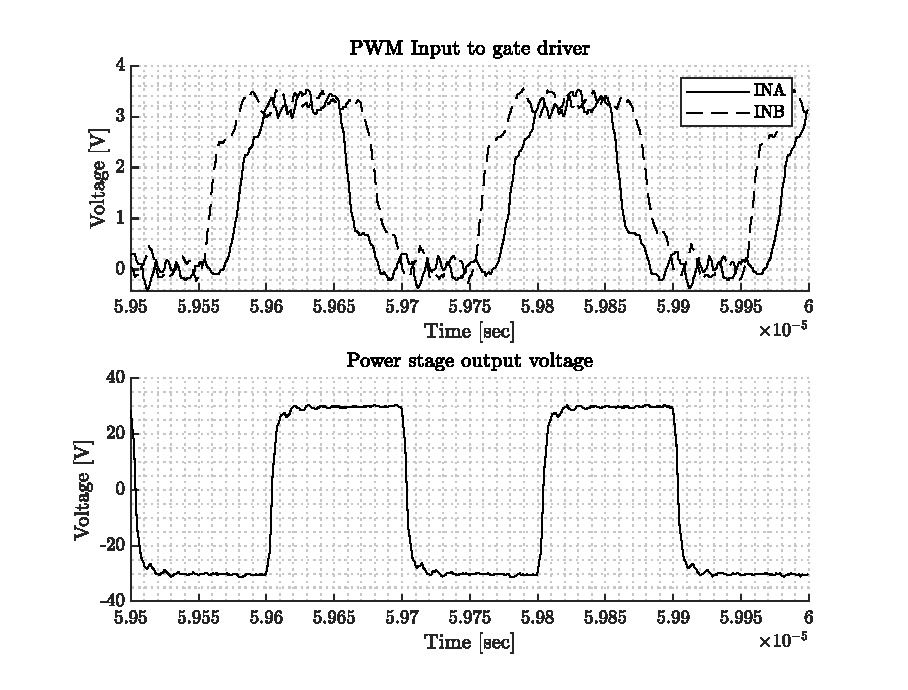
\includegraphics[width=.8\textwidth]{Figures/4_transmitter_pcb_out.eps}
	\caption[Measured input and output of power stage PCB]{Measured input and output of power stage PCB. (Above) Input to gate driver with dead-time (Below) Output of MOSFET half-bridge and the voltage across the load}
	\label{fig:4_transmitter_meas}
\end{figure}

\subsection{Transmit/Receive Switch}
\begin{figure}[htbp]
	\centering
	\includegraphics[width=.8\textwidth]{Figures/4_switch_meas_pic.jpg}
	\caption{TX/RX Switch reflection experiment with water tank}
	\label{fig:4_switch_meas_pic}
\end{figure}
For validating the TX/RX switch, an experiment is conducted with a \gls{pzt} transducer, water tank, function generator and an oscilloscope. Using two input signals, $f_{\mathrm{prf}}=\qty{10}{\kilo\hertz}$ switch signal, and $f_{0}=\qty{5}{\mega\hertz}$ burst mode transmit signal, the switch is configured to transmit and receive. A picture of the submerged transducer with a reflector can be seen in \cref{fig:4_switch_meas_pic}. After submerging the transducer in distilled water and measuring on the receiver side of the TX/RX switch, a reflected signal from the tank can be observed in \cref{fig:4_txrx_meas}.
\begin{figure}[htbp]
	\centering
	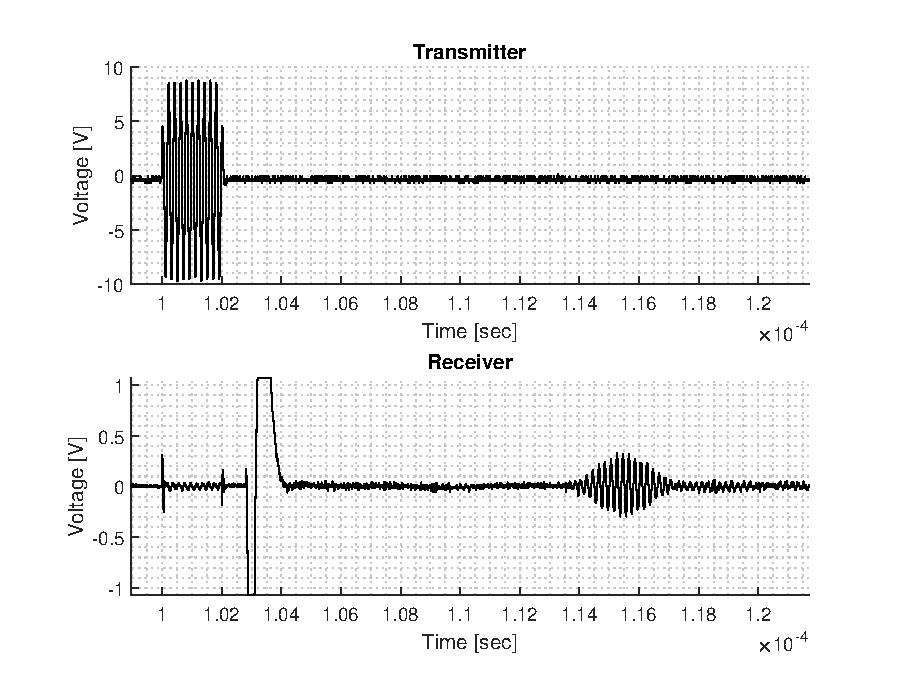
\includegraphics[width=.8\textwidth]{Figures/4_switch_pcb_meas.eps}
	\caption[Measured transmit and receive on Transmit/Receive Switch PCB]{Measured transmit and receive on Transmit/Receive Switch PCB (Above) Measured transmit voltage (Below) Received reflected signal off water tank}
	\label{fig:4_txrx_meas}
\end{figure}

\subsection{Band-pass Filter}
it is desired to validate its frequency response to determine if it functions as desired. To obtain the frequency response, a bode plot of the magnitude and phase is measured from \qty{300}{\kilo\hertz} until \qty{20}{\mega\hertz} using a \gls{vna} in a S21 configuration, meaning a measurement of the output in respect to the input. This measurement determines the difference in magnitude and phase of the output in comparison with the input signal. Observed in \cref{fig:4_bpf_measurement} is the frequency response of the band-pass filter measured on a \gls{vna}. It is noted that the pass band frequencies are mostly as expected with \qty{-0.5}{\decibel} frequencies at \qty{1.5}{\mega\hertz} and \qty{7}{\mega\hertz}. Though, the roll-off in the higher stop band appears somewhat lower than in the lower stop band. That would mean that it is plausible that higher frequency noise components are retained in the output than in the lower stop band. For the phase, it seems to have a significant phase delay, going from around \qty{100}{\degree} to \qty{250}{\degree} from the start to the end of the pass band.
\begin{figure}[htbp]
	\centering
	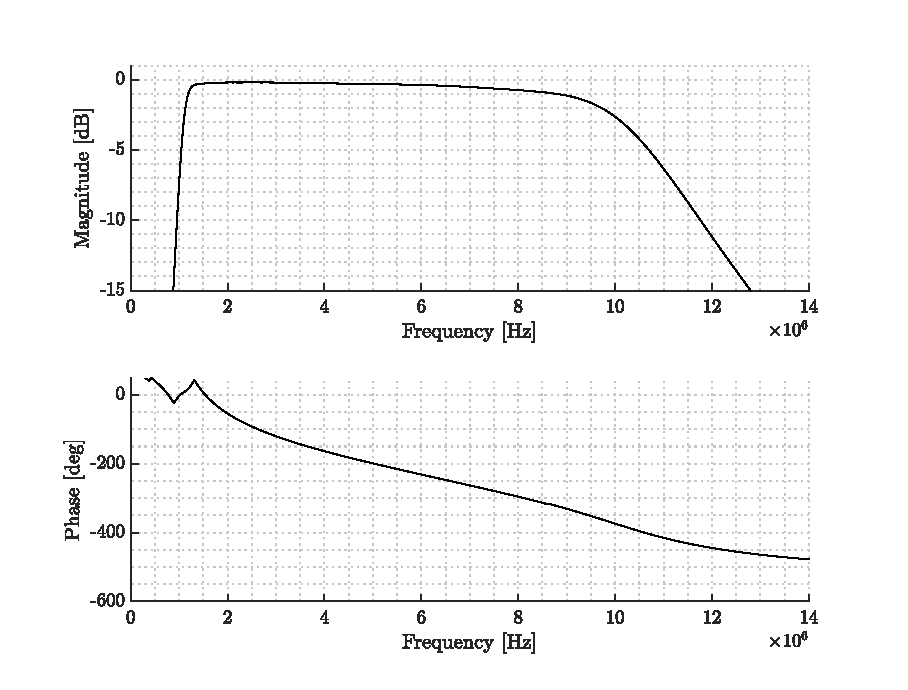
\includegraphics[width=.8\textwidth]{Figures/4_bpf_measurement_vna.eps}
	\caption[Band-pass filter bode plot]{Band-pass Filter bode plot from \qtyrange{0.3}{14}{\mega\hertz} with (above) magnitude and (below) phase}
	\label{fig:4_bpf_measurement}
\end{figure}

\subsection{Preamplifier}
Seen in \cref{fig:4_preamp_in} are measurements of the preamplifier circuits showing a \qty{70}{\milli\volt} input signal and a \qty{300}{\milli\volt} output signal with a \qty{2.5}{\volt} DC bias. In this application, however, only the \gls{lna} is used, and the \gls{vga} is bypassed in the hardware preamplifier configuration. The schematic of the preamplifier circuit is part of the demodulation schematic and can be found in the appendix in \cref{fig:appendix_ad8333}.
\begin{figure}[htbp]
	\centering
	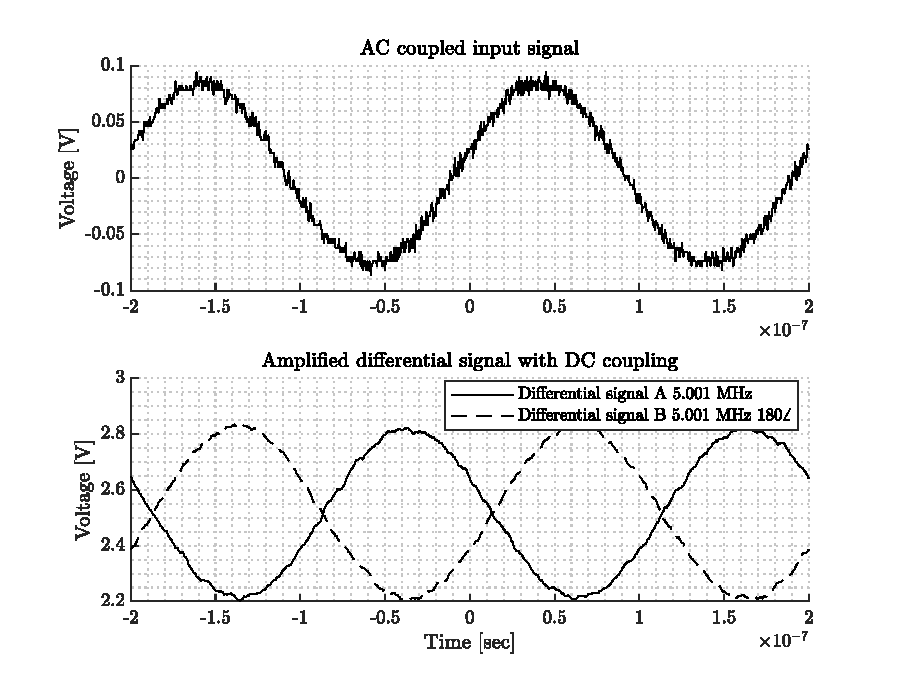
\includegraphics[width=.8\textwidth]{Figures/4_preamplifier_pcb.eps}
	\caption[Measured input and output of preamplifier PCB]{Measured input of preamplifier PCB, (Above) AC coupled input signal with amplitude \qty{1}{\volt} (Below Measured output of preamplifier PCB, Differential signal with DC coupling and $\times \qty{19}{\decibel}$ amplification)}
	\label{fig:4_preamp_in}
\end{figure}

\subsection{Demodulator}
An experiment is conducted with the sample-and-hold amplifier to verify the functionality. A low-frequency I-Q simulated signal is created from the function generator with a sample gating pulse train to control the sample-and-hold function. Seen in \cref{fig:4_demod_in} are the input signals, differential signals of \qty{5.001}{\mega\hertz} and \qty{20}{\mega\hertz} local oscillator signal. Seen in \cref{fig:4_demod_out} are the differential input signals $A$ and $B$ and the demodulated output signals $I$ and $Q$, where the phase between $I$ and $Q$ denotes the Doppler shift direction, or rather, the direction of flow of the scatterer. It is noted that the differential signal is so high frequency compared to the timescale so there has to be a zoomed in subplot where the waveform is visible to show the waveform. This highlights the observation of the Doppler shift being pushed down in frequency, which is one of the key functions of the demodulator in this system.

\begin{figure}[htbp]
	\centering
	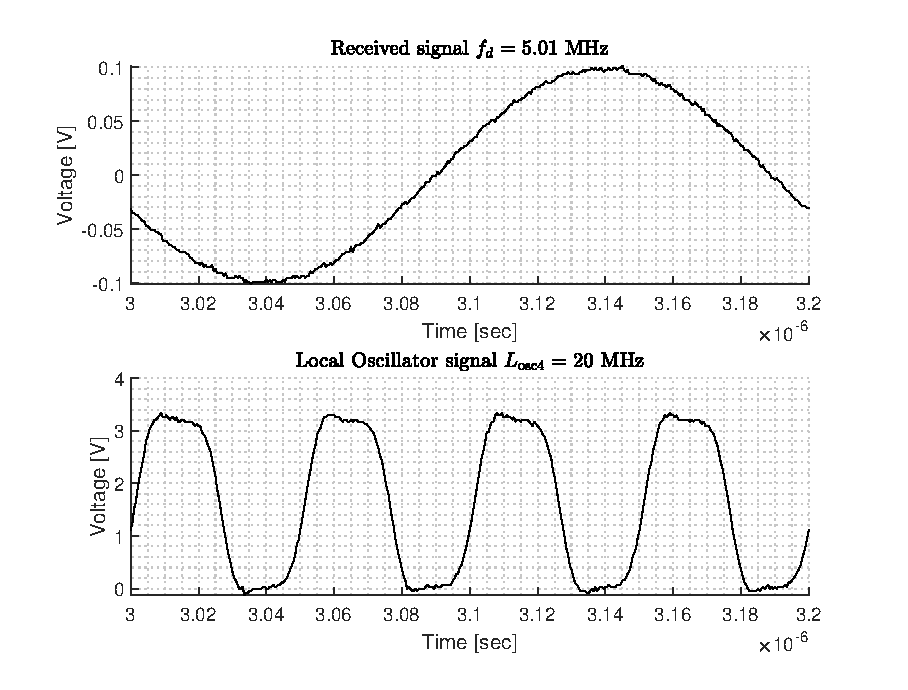
\includegraphics[width=.8\textwidth]{Figures/4_demod_pcb_in.eps}
	\caption[Measured input of demodulator PCB]{Measured input of demodulator PCB (Above) Input from received signal (Below) Input from local oscillator ($f_{0}\cdot4$)}
	\label{fig:4_demod_in}
\end{figure}
\begin{figure}[htbp]
	\centering
	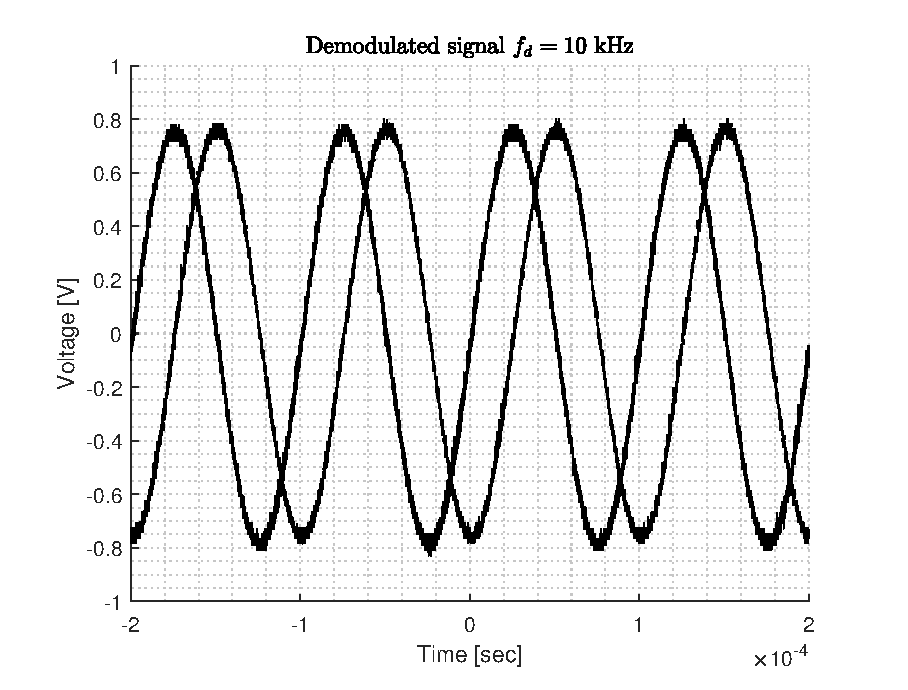
\includegraphics[width=.8\textwidth]{Figures/4_demod_pcb_out.eps}
	\caption[Measured output of demodulator PCB]{Measured output of demodulator PCB}
	\label{fig:4_demod_out}
\end{figure}

\subsection{Sample and Hold Amplifier}
Seen in \cref{fig:4_sample_hold_pcb} is the measured inputs and outputs of the circuit during the experiment. Above is the I-Q input and in the middle is the sample gating, and below is the output signal. On the output signal, it is noted the corresponding voltage transients for every pulse in the gate input.
\begin{figure}[htbp]
	\centering
	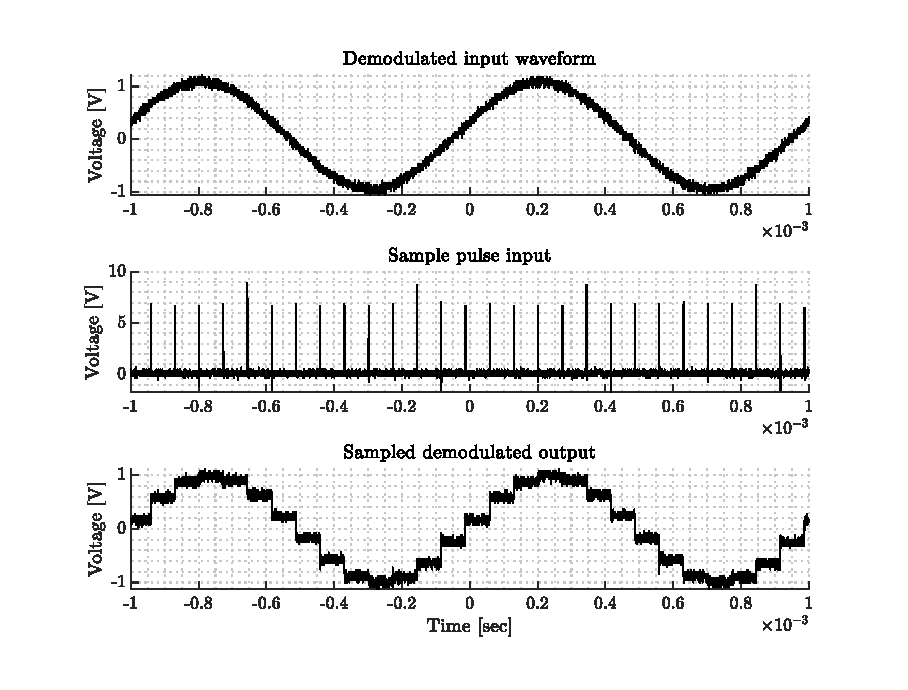
\includegraphics[width=.8\textwidth]{Figures/4_sampler_pcb.eps}
	\caption{Measured input and output of Sample and Hold amplifier}
	\label{fig:4_sample_hold_pcb}
\end{figure}

\subsection{Active Filter}
\begin{figure}
	\centering
	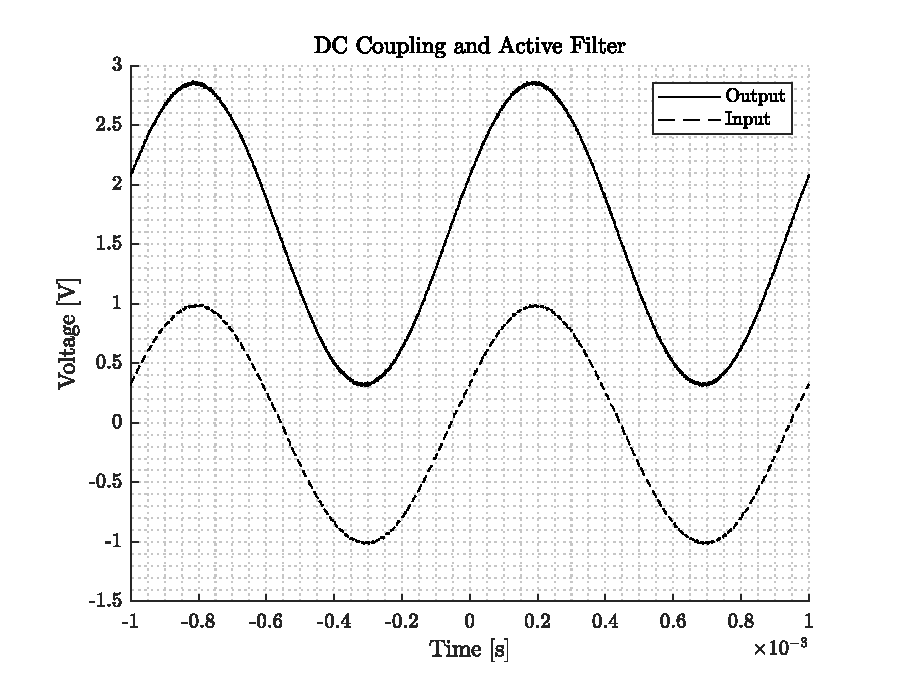
\includegraphics[width=.8\textwidth]{Figures/5_dccoupler_filter_measurement.eps}
	\caption{Measured input and output of Active filter and DC Coupler}
	\label{fig:5_dccoupler_measured}
\end{figure}
A \qty{1}{\kilo\hertz} input signal is received on the input SMA connector from a function generator and probed with an oscilloscope. $\pm\qty{5}{\volt}$ is supplied to the power terminals. Next, the output SMA connector is probed with an oscilloscope and the data is recorded. The dashed line is the \gls{ac} coupled input signal with \qty{1}{\volt} amplitude and the solid line is the amplified \gls{dc} coupled output signal. Seen in \cref{fig:5_dccoupler_measured} is the measured input and output of the DC coupler and active filter. This measurement confirms its operation as expected when comparing to the simulation shown earlier in the report.

\subsection{Digital Signal Processor}
A function generator is configured to transmit a \qty{100}{\hertz} sinusoidal signal with a \qty{0.5}{\volt} offset and a \qty{1}{\volt} peak-peak amplitude. This signal is then measured by the DSP XADC and saved for processing. A peak samplerate is determined by recording the maximum amount of samples possible but limiting the collection time to one second. Then, the samplerate is identical to the number of samples collected. After one second of sampling, a record of 4422 samples were stored in the buffer.
\begin{figure}[htbp]
	\centering
	\includegraphics[width=.8\textwidth]{Figures/5_velocity_estimation_measured.pdf}
	\caption{Velocity estimation with XADC and Jupyter}
	\label{fig:5_velocity_estimation_output}
\end{figure}
After processing the data, a total of three plots are generated and can be seen in \cref{fig:5_velocity_estimation_output}. In the top plot, the whole buffer is plotted over time. In the middle plot, the spectrum of the recorded measurements are plotted. In the lower plot, two periods of the largest frequency components are plotted.
\begin{figure}[htbp]
	\centering
	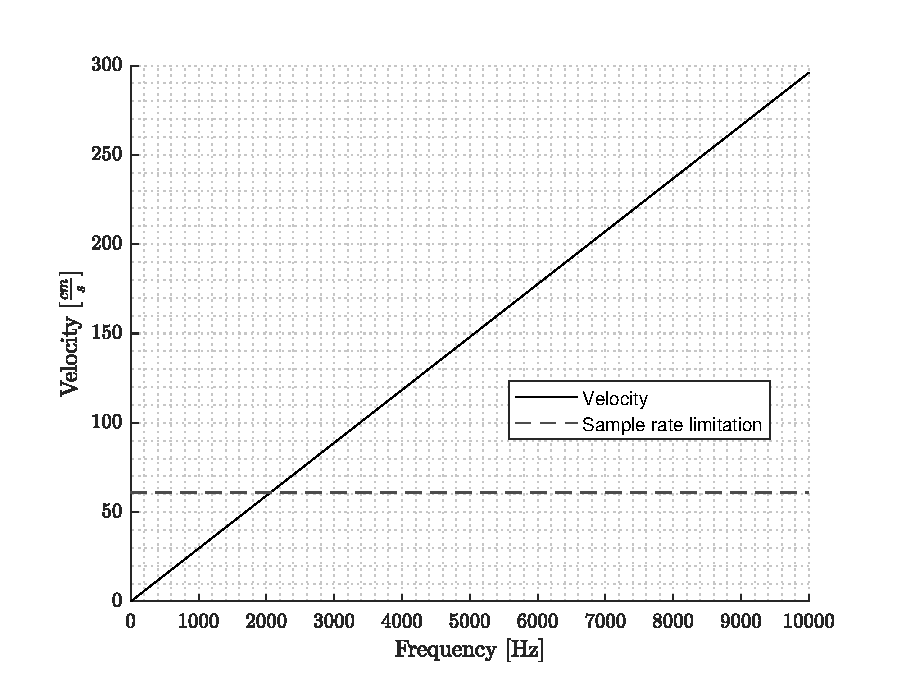
\includegraphics[width=.8\textwidth]{Figures/5_velocity_estimation_limit.eps}
	\caption{Velocity estimator with sample rate limitation}
	\label{fig:5_dsp_samplerate_limit}
\end{figure}
Since the maximum sample rate with the XADC implementation used was determined, it is desired to know the limitations of the Doppler velocity estimation. Based on the Nyquist limit, a with 0.5 cycle/sample results in distortion known as aliasing. In principle, it means that when the same rate was determined to be 4422 samples per second, that means the Nyquist frequency for this system is equal to \qty{2211}{\hertz}. In the application of a velocity estimator, that means that a velocity of over \qty{60}{\centi\meter\per\second} will result in high distortion and unreliable measurements.

\section{Pulse Generator and Power Stage}
Using the pulse generator and the power stage, an experiment is performed where the complementary PWM signals are generated and output to the gate driver of the power stage. In turn, the gate driver will drive the MOSFET pair and output a high-power output than the pulse generator can supply on its own through its \gls{gpio}.

\begin{figure}[htbp]
	\centering
	\includegraphics[width=.8\textwidth]{Figures/5_controlsystem_fpga_pwm.png}
	\caption{Complementary PWM output from the pulse generator and bipolar high power pulses}
	\label{fig:5_pulse_generator_experiment}
\end{figure}

Seen in \cref{fig:5_pulse_generator_experiment} are the measurements obtained from the pulse generator and power stage experiment. The measurements show the ability of the Pynq Z1 as a pulse generator is functioning as expected. As the power stage half-bridge is rail-to-rail, the output pulse voltages depend on the power supply voltage. In this case, the experiment is using a \qty{30}{\volt} maximum \gls{dcps}, and the output peak pulse voltages are $\pm \qty{30}{\volt}$. However, the power stage itself is specified for bipolar operating voltages up to $\pm \qty{100}{\volt}$, or unipolar voltages $\pm \qty{200}{\volt}$.

\section{Doppler String Phantom Experiment}
\begin{figure}[htbp]
	\centering
	\includegraphics[width=.8\textwidth]{Figures/5_cirs_043a_image.jpg}
	\caption[CIRS Model 043A Doppler String Phantom]{CIRS Model 043A Doppler String Phantom with (left) motor controller and (right) tank and string loop}
	\label{fig:5_doppler_string_phantom}
\end{figure}
Seen in \cref{fig:5_doppler_string_phantom} is the CIRS A043 Doppler String Phantom is a device used to evaluate the performance of Doppler ultrasound imaging systems. The phantom consists of a string that is driven by a motor. The motor can be programmed to move at different speeds and directions, and can also be configured to drive the string with physiological waveforms, such as a carotid artery for validation purposes. A Doppler string phantom validation technique is widely used in research, development, and quality assurance of Doppler ultrasound equipment.
\begin{figure}[htbp]
	\centering
%	\begin{adjustbox}{width=\textwidth}%
%		

\tikzset{every picture/.style={line width=0.75pt}} %set default line width to 0.75pt

\begin{tikzpicture}[x=0.75pt,y=0.75pt,yscale=-1,xscale=1]
	%uncomment if require: \path (0,244); %set diagram left start at 0, and has height of 244

	%Shape: Rectangle [id:dp6722494395467095]
	\draw  [fill={rgb, 255:red, 74; green, 144; blue, 226 }  ,fill opacity=0.43 ][dash pattern={on 0.84pt off 2.51pt}] (40,120) -- (260,120) -- (260,200) -- (40,200) -- cycle ;
	%Shape: Rectangle [id:dp07000140128396126]
	\draw  [fill={rgb, 255:red, 74; green, 74; blue, 74 }  ,fill opacity=1 ] (140,40) -- (200,40) -- (200,80) -- (140,80) -- cycle ;
	%Shape: Circle [id:dp1435775000611489]
	\draw  [fill={rgb, 255:red, 128; green, 128; blue, 128 }  ,fill opacity=1 ] (240,190) .. controls (240,184.48) and (244.48,180) .. (250,180) .. controls (255.52,180) and (260,184.48) .. (260,190) .. controls (260,195.52) and (255.52,200) .. (250,200) .. controls (244.48,200) and (240,195.52) .. (240,190) -- cycle ;
	%Straight Lines [id:da5994952267655665]
	\draw    (50,70) -- (50,150) (54,80) -- (46,80)(54,90) -- (46,90)(54,100) -- (46,100)(54,110) -- (46,110)(54,120) -- (46,120)(54,130) -- (46,130)(54,140) -- (46,140) ;
	%Shape: Rectangle [id:dp7130303275600529]
	\draw  [color={rgb, 255:red, 0; green, 0; blue, 0 }  ,draw opacity=1 ][fill={rgb, 255:red, 128; green, 128; blue, 128 }  ,fill opacity=1 ] (40,60) -- (60,60) -- (60,80) -- (40,80) -- cycle ;
	%Shape: Circle [id:dp883251536454338]
	\draw  [fill={rgb, 255:red, 0; green, 0; blue, 0 }  ,fill opacity=1 ] (45,162.5) .. controls (45,152.84) and (52.84,145) .. (62.5,145) .. controls (72.16,145) and (80,152.84) .. (80,162.5) .. controls (80,172.16) and (72.16,180) .. (62.5,180) .. controls (52.84,180) and (45,172.16) .. (45,162.5) -- cycle ;
	%Shape: Rectangle [id:dp3769942512437483]
	\draw   (40,160) -- (60,160) -- (60,180) -- (40,180) -- cycle ;
	%Shape: Circle [id:dp8079321779320666]
	\draw  [dash pattern={on 3.75pt off 3pt on 7.5pt off 1.5pt}] (240,190) .. controls (240,184.48) and (244.48,180) .. (250,180) .. controls (255.52,180) and (260,184.48) .. (260,190) .. controls (260,195.52) and (255.52,200) .. (250,200) .. controls (244.48,200) and (240,195.52) .. (240,190) -- cycle ;
	%Straight Lines [id:da7273832971820673]
	\draw    (60,180) -- (250,200) (70.36,177.07) -- (69.53,185.02)(80.31,178.12) -- (79.47,186.07)(90.25,179.16) -- (89.42,187.12)(100.2,180.21) -- (99.36,188.17)(110.14,181.26) -- (109.31,189.21)(120.09,182.3) -- (119.25,190.26)(130.03,183.35) -- (129.2,191.31)(139.98,184.4) -- (139.14,192.35)(149.92,185.44) -- (149.09,193.4)(159.87,186.49) -- (159.03,194.45)(169.81,187.54) -- (168.98,195.49)(179.76,188.58) -- (178.92,196.54)(189.7,189.63) -- (188.87,197.59)(199.65,190.68) -- (198.81,198.63)(209.59,191.72) -- (208.76,199.68)(219.54,192.77) -- (218.7,200.73)(229.48,193.82) -- (228.65,201.77)(239.43,194.87) -- (238.59,202.82)(249.37,195.91) -- (248.54,203.87) ;
	%Straight Lines [id:da05910308874228931]
	\draw    (70,160) -- (250,180) (80.38,157.13) -- (79.5,165.08)(90.32,158.23) -- (89.44,166.18)(100.26,159.34) -- (99.37,167.29)(110.2,160.44) -- (109.31,168.39)(120.14,161.55) -- (119.25,169.5)(130.07,162.65) -- (129.19,170.6)(140.01,163.75) -- (139.13,171.71)(149.95,164.86) -- (149.07,172.81)(159.89,165.96) -- (159.01,173.91)(169.83,167.07) -- (168.95,175.02)(179.77,168.17) -- (178.89,176.12)(189.71,169.28) -- (188.82,177.23)(199.65,170.38) -- (198.76,178.33)(209.59,171.48) -- (208.7,179.44)(219.52,172.59) -- (218.64,180.54)(229.46,173.69) -- (228.58,181.64)(239.4,174.8) -- (238.52,182.75)(249.34,175.9) -- (248.46,183.85) ;
	%Straight Lines [id:da12196496059097228]
	\draw [fill={rgb, 255:red, 0; green, 0; blue, 0 }  ,fill opacity=1 ]   (70,70) -- (70,160) (74,80) -- (66,80)(74,90) -- (66,90)(74,100) -- (66,100)(74,110) -- (66,110)(74,120) -- (66,120)(74,130) -- (66,130)(74,140) -- (66,140)(74,150) -- (66,150) ;
	%Curve Lines [id:da7394389878662597]
	\draw  [dash pattern={on 0.75pt off 0.75pt}]  (160,140) .. controls (162.22,141.07) and (162.72,142.66) .. (161.49,144.77) .. controls (159.76,145.92) and (159.25,147.46) .. (159.97,149.41) .. controls (159.98,151.75) and (158.86,152.97) .. (156.59,153.07) .. controls (154.34,154.26) and (153.98,155.87) .. (155.53,157.88) -- (155.94,160.34) -- (158.75,167.6) ;
	\draw [shift={(160,170)}, rotate = 241.56] [fill={rgb, 255:red, 0; green, 0; blue, 0 }  ][line width=0.08]  [draw opacity=0] (10.72,-5.15) -- (0,0) -- (10.72,5.15) -- (7.12,0) -- cycle    ;
	%Curve Lines [id:da9786153302440782]
	\draw  [dash pattern={on 0.75pt off 0.75pt}]  (175.5,170) .. controls (173.28,168.93) and (172.78,167.34) .. (174,165.23) .. controls (175.74,164.08) and (176.25,162.54) .. (175.53,160.59) .. controls (175.52,158.25) and (176.64,157.03) .. (178.91,156.93) .. controls (181.16,155.74) and (181.51,154.13) .. (179.97,152.12) -- (179.56,149.66) -- (176.74,142.4) ;
	\draw [shift={(175.5,140)}, rotate = 61.56] [fill={rgb, 255:red, 0; green, 0; blue, 0 }  ][line width=0.08]  [draw opacity=0] (10.72,-5.15) -- (0,0) -- (10.72,5.15) -- (7.12,0) -- cycle    ;
	%Straight Lines [id:da7205891380538312]
	\draw [color={rgb, 255:red, 128; green, 128; blue, 128 }  ,draw opacity=1 ]   (80,90) -- (80,117) ;
	\draw [shift={(80,120)}, rotate = 270] [fill={rgb, 255:red, 128; green, 128; blue, 128 }  ,fill opacity=1 ][line width=0.08]  [draw opacity=0] (8.93,-4.29) -- (0,0) -- (8.93,4.29) -- cycle    ;
	%Straight Lines [id:da631680111682684]
	\draw [color={rgb, 255:red, 128; green, 128; blue, 128 }  ,draw opacity=1 ]   (60,93) -- (60,120) ;
	\draw [shift={(60,90)}, rotate = 90] [fill={rgb, 255:red, 128; green, 128; blue, 128 }  ,fill opacity=1 ][line width=0.08]  [draw opacity=0] (8.93,-4.29) -- (0,0) -- (8.93,4.29) -- cycle    ;
	%Shape: Polygon [id:ds5396773368746502]
	\draw  [fill={rgb, 255:red, 255; green, 255; blue, 255 }  ,fill opacity=1 ] (40,60) -- (40,200) -- (260,200) -- (260,100) -- (280,100) -- (280,220) -- (20,220) -- (20,60) -- cycle ;
	%Shape: Circle [id:dp9531409722820131]
	\draw  [fill={rgb, 255:red, 155; green, 155; blue, 155 }  ,fill opacity=1 ] (50,70) .. controls (50,61.72) and (56.72,55) .. (65,55) .. controls (73.28,55) and (80,61.72) .. (80,70) .. controls (80,78.28) and (73.28,85) .. (65,85) .. controls (56.72,85) and (50,78.28) .. (50,70) -- cycle ;
	%Straight Lines [id:da9454073791401769]
	\draw [fill={rgb, 255:red, 255; green, 255; blue, 255 }  ,fill opacity=1 ]   (280,150) -- (280,100) -- (220,40) -- (140,40) -- (140,30) -- (230,30) -- (280,80) -- (300,80) -- (300,150) -- cycle ;

	% Text Node
	\draw  [fill={rgb, 255:red, 255; green, 255; blue, 255 }  ,fill opacity=1 ]  (156.5,58.5) -- (182.5,58.5) -- (182.5,139.5) -- (156.5,139.5) -- cycle  ;
	\draw (169.5,99) node  [rotate=-270] [align=left] {{\fontfamily{pcr}\selectfont Transducer}};
	% Text Node
	\draw  [fill={rgb, 255:red, 255; green, 255; blue, 255 }  ,fill opacity=1 ]  (361,18) -- (442,18) -- (442,65) -- (361,65) -- cycle  ;
	\draw (401.5,41.5) node   [align=left] {\begin{minipage}[lt]{52.33pt}\setlength\topsep{0pt}
			\begin{center}
				{\fontfamily{pcr}\selectfont Ultrasound}\\{\fontfamily{pcr}\selectfont Switch}
			\end{center}

	\end{minipage}};
	% Text Node
	\draw  [fill={rgb, 255:red, 255; green, 255; blue, 255 }  ,fill opacity=1 ]  (478,18) -- (526,18) -- (526,65) -- (478,65) -- cycle  ;
	\draw (502,41.5) node   [align=left] {\begin{minipage}[lt]{29.8pt}\setlength\topsep{0pt}
			\begin{center}
				{\fontfamily{pcr}\selectfont Power}\\{\fontfamily{pcr}\selectfont Stage}
			\end{center}

	\end{minipage}};
	% Text Node
	\draw  [fill={rgb, 255:red, 255; green, 255; blue, 255 }  ,fill opacity=1 ]  (566.5,17.5) -- (647.5,17.5) -- (647.5,64.5) -- (566.5,64.5) -- cycle  ;
	\draw (607,41) node   [align=left] {\begin{minipage}[lt]{52.33pt}\setlength\topsep{0pt}
			\begin{center}
				{\fontfamily{pcr}\selectfont Ultrasound}\\{\fontfamily{pcr}\selectfont Pulser}
			\end{center}

	\end{minipage}};
	% Text Node
	\draw  [fill={rgb, 255:red, 255; green, 255; blue, 255 }  ,fill opacity=1 ]  (358,98) -- (446,98) -- (446,124) -- (358,124) -- cycle  ;
	\draw (402,111) node   [align=left] {\begin{minipage}[lt]{57.26pt}\setlength\topsep{0pt}
			\begin{center}
				{\fontfamily{pcr}\selectfont Preamplifier}
			\end{center}

	\end{minipage}};
	% Text Node
	\draw  [fill={rgb, 255:red, 255; green, 255; blue, 255 }  ,fill opacity=1 ]  (478,98) -- (572,98) -- (572,124) -- (478,124) -- cycle  ;
	\draw (525,111) node   [align=left] {\begin{minipage}[lt]{61.2pt}\setlength\topsep{0pt}
			\begin{center}
				{\fontfamily{pcr}\selectfont Demodulator}
			\end{center}

	\end{minipage}};
	% Text Node
	\draw  [fill={rgb, 255:red, 255; green, 255; blue, 255 }  ,fill opacity=1 ]  (604,98) -- (692,98) -- (692,124) -- (604,124) -- cycle  ;
	\draw (648,111) node   [align=left] {\begin{minipage}[lt]{56.9pt}\setlength\topsep{0pt}
			\begin{center}
				{\fontfamily{pcr}\selectfont Oscilloscope}
			\end{center}

	\end{minipage}};
	% Connection
	\draw    (478,41.5) -- (444,41.5) ;
	\draw [shift={(442,41.5)}, rotate = 360] [color={rgb, 255:red, 0; green, 0; blue, 0 }  ][line width=0.75]    (10.93,-3.29) .. controls (6.95,-1.4) and (3.31,-0.3) .. (0,0) .. controls (3.31,0.3) and (6.95,1.4) .. (10.93,3.29)   ;
	% Connection
	\draw    (566.5,41.19) -- (528,41.38) ;
	\draw [shift={(526,41.39)}, rotate = 359.73] [color={rgb, 255:red, 0; green, 0; blue, 0 }  ][line width=0.75]    (10.93,-3.29) .. controls (6.95,-1.4) and (3.31,-0.3) .. (0,0) .. controls (3.31,0.3) and (6.95,1.4) .. (10.93,3.29)   ;
	% Connection
	\draw    (401.67,65) -- (401.89,96) ;
	\draw [shift={(401.91,98)}, rotate = 269.59] [color={rgb, 255:red, 0; green, 0; blue, 0 }  ][line width=0.75]    (10.93,-3.29) .. controls (6.95,-1.4) and (3.31,-0.3) .. (0,0) .. controls (3.31,0.3) and (6.95,1.4) .. (10.93,3.29)   ;
	% Connection
	\draw    (446,111) -- (476,111) ;
	\draw [shift={(478,111)}, rotate = 180] [color={rgb, 255:red, 0; green, 0; blue, 0 }  ][line width=0.75]    (10.93,-3.29) .. controls (6.95,-1.4) and (3.31,-0.3) .. (0,0) .. controls (3.31,0.3) and (6.95,1.4) .. (10.93,3.29)   ;
	% Connection
	\draw    (572,111) -- (602,111) ;
	\draw [shift={(604,111)}, rotate = 180] [color={rgb, 255:red, 0; green, 0; blue, 0 }  ][line width=0.75]    (10.93,-3.29) .. controls (6.95,-1.4) and (3.31,-0.3) .. (0,0) .. controls (3.31,0.3) and (6.95,1.4) .. (10.93,3.29)   ;
	% Connection
	\draw    (357.41,49.38) .. controls (312.15,51.65) and (308.79,102.38) .. (184.38,99.26) ;
	\draw [shift={(182.5,99.21)}, rotate = 1.67] [fill={rgb, 255:red, 0; green, 0; blue, 0 }  ][line width=0.08]  [draw opacity=0] (8.93,-4.29) -- (0,0) -- (8.93,4.29) -- cycle    ;
	\draw [shift={(361,49.3)}, rotate = 180.36] [fill={rgb, 255:red, 0; green, 0; blue, 0 }  ][line width=0.08]  [draw opacity=0] (8.93,-4.29) -- (0,0) -- (8.93,4.29) -- cycle    ;

\end{tikzpicture}

%	\end{adjustbox}%
	\includegraphics[width=\textwidth]{Figures/5_doppler_string_phantom_experiment.pdf}
	\caption{Doppler String Phantom experiment diagram (not to scale)}
	\label{fig:5_doppler_string_experiment}
\end{figure}
In \cref{fig:5_doppler_string_experiment} is a diagram of the experiment to be performed with the analogue front-end to evaluate the performance of the system. The ultrasound system is being controlled by the ultrasound pulser running on the PYNQ-Z1 board. The transducer used in the experiment is a piezoelectric \qty{5}{\mega\hertz} commercial transducer. The entire system operates at a \texttt{PRF} frequency of \qty{15}{\kilo\hertz}. First, the string is mounted in the string phantom loop. Next, the transducer is mounted on a movable arm and submerged in the water. When the ultrasound waves strike the moving string, the frequency of the reflected waves is shifted due to the Doppler effect. This frequency shift provides information about the velocity and direction of the simulated blood flow. Here, the ultrasound system measures the frequency shift and this can in turn be calculated into a velocity. This data can be analyzed to assess the accuracy and performance of the Doppler ultrasound system. The phantom allows for calibration of the system and evaluation of factors such as velocity sensitivity, and spectral Doppler analysis when looking at the \gls{psd} over time. Unfortunately, when conducting the experiment, a design review indicated that the pulser required a modification to the output of the power stage to ensure the potential across the transducer is bled off during rest. However, this must be carefully balanced to ensure that an increased load is not attenuating the received signal. Two solutions were proposed:
\begin{enumerate}
	\item A resistor to reference voltage in parallel with the transducer
	\item A second ultrasound switch, functionally inverse of the primary ultrasound switch to ensure received signal does not get attenuated by pulser circuit
\end{enumerate}
	\chapter{Conclusion}
In conclusion, this project has successfully gone through thorough research, data collection, and analysis, and have obtained a comprehensive understanding of the subject matter. Through a literature review, key gaps in the research have been identified. This formed the basis of a design approach to the ultrasound system that was followed throughout the project. This project aimed to design, build, and test an ultrasound system for blood velocity estimation that can be miniaturised. The implementation of all the sub-components in the system was simulated and/or tested thoroughly to verify the function. Moreover, some of the combined testing revealed some implementation changes necessary in the power stage output. Despite the numerous achievements and contributions made throughout this project, it is important to acknowledge its limitations. Factors such as time constraints, limited resources, and external factors beyond our control may have impacted the scope and depth of our study. However, the findings and insights presented in this report should provide a solid foundation for future research and further exploration of the topic. Due to time limitations, experiments were focused on module testing each part of the system independently. It is therefore difficult to compare it with prior research directly. The system was designed around a control system based on the Zynq 7000 SoC, which contains both the configured ultrasound pulser logic controller and the Python-based programmable interface. The transmitter, which includes the ultrasound pulser and the power stage, was tested with the switch, and while the transmitting was successful, a received reflected signal could not be found. It is believed that the received switch was sinking into the on-board load of the power stage.  On the receiver, which includes the bandpass filter, preamplifier, quadrature demodulator, sample and hold circuit, and active filter, were also verified functioning as intended in isolated experiments. The implementation of the analogue frontend can result in a more compact commercial product. However, more work is required before a working single-device prototype can be build and evaluated.
\section{Future Work}
The system was fully validated, although in module testing. The absence of reflected signals, when using the  power stage, should be further investigated. In the future, it is desired to perform a complete system test and evaluate the performance using the physiological simulator. After a successful experiment, a single PCB layout can be completed from the CAD work already done for the documentation in Altium Designer. Another future work would be further implementing a continuous data acquisition with a spectral image, thus fully displaying the sonographic data in the DSP.
%
	\printbibliography[heading=bibintoc,title={Bibliography}]
	%%
	%% 감사의 글 시작
	%% Acknowledgement
	%%
	% @command acknowledgement 감사의글
	% @options [1 | 2 | 3 |4 ]
	% - 1 : 본문과 감사의 글이 둘 다 한글일 때  | 2 : 본문은 한글인데 감사의 글이 영어일 때 | 3 :  본문과 감사의 글이 둘 다 영어일 때  | 4 : 본문은 영어인데 감사의 글이 % 한글일 때
	%% It is optional.

	\acknowledgment[4]
%	언제나 저를 바른 길로 이끌어 주시는 송익호 교수님께 큰 고마움을 느낍니다.
%	끝으로 오늘의 제가 있을 수 있도록 사랑으로 키워 주신 가족들에게 감사드립니다.
%	저의 이 작은 결실이 그분들께 조금이나마 보답이 되기를 바랍니다.

	%%
	%% 약력 시작
	%% Curriculum Vitae
	%%
	% @command curriculumvitae 이력서
	% @options [1 | 2 | 3 |4 ]
	% - 1 : 본문과 약력이 둘 다 한글일 때  | 2 : 본문은 한글인데 약력이 영어일 때 | 3 :  본문과 약력이 둘 다 영어일 때  | 4 : 본문은 영어인데 약력이 한글일 때
	%% It is optional and you can change form of this in the class file if you want.
	\curriculumvitae[4]

	% @environment personaldata 개인정보
	% @command     name         이름
	%              dateofbirth  생년월일
	%              birthplace   출생지
	%              domicile     본적지
	%              address      주소지
	%              email        E-mail 주소
	% - 위 6개의 기본 필드 중에 이력서에 적고 싶은 정보를 입력
	% input data only you want
	\begin{personaldata}
		\name       {힌릭스 예폐}
		\dateofbirth{1991}{07}{22}
		\birthplace {오르후스 덴마크}
		\address    {대전, 대한민국}
	\end{personaldata}

	% @environment education 학력
	% @options [default: (none)] - 수학기간을 입력
	\begin{education}
		\item[2018. 2.\ --\ 2021. 1.] Technical University of Denmark 전기및전자공학부 (학사)
		\item[2020. 2.\ --\ 2020. 8.] Tokyo Institute of Technology 전기및전자공학부 (교환학생)
		\item[2021. 2.\ --\ 2023. 6.] Technical University of Denmark 전기및전자공학부 (석사)
		\item[2021. 8.\ --\ 2023. 8.] 한국과학기술원 전기및전자공학부 (석사)
	\end{education}

	% @environment career 경력
	% @options [default: (none)] - 해당기간을 입력
	\begin{career}
		\item[2015. 7.\ --\ 2017. 8.] Welltec A/S 테스트 공학자
		\item[2018. 9.\ --\ 2021. 6.] Technical University of Denmark 국립 우주 연구소 조교
	\end{career}

	% @environment activity 학회활동
	% @options [default: (none)] - 활동내용을 입력
	%%    \begin{activity}
		%%        \item J. Choi, \textbf{Yong-Hyun Kim}, K.J. Chang, and D. Tomanek,
		%%             \textit{Occurrence of itinerant ferromagnetism in C/BN superlattice
			%%             nanotubes}, 5th Asian Workshop on First-Principles Electronic
		%%             Structure Calculations, Seoul (Korea), October., 2002.
		%%    \end{activity}

	% @environment publication 연구업적
	% @options [default: (none)] - 출판내용을 입력
%	\begin{publication}
%		%\item \textbf{Yong-Hyun Kim}, J. Choi, K.J. Chang, and D. Tomanek,
%		%     \textit{Magnetic instability in partly opened C$_{60}$ isomers},
%		%     in preparation.
%		\item H.-K. Min, Y. Hou, {\bf S. Park}, and I. Song,
%		``A computationally efficient scheme for feature extraction with kernel discriminant analysis,"
%		\textit{Patt. Recogn.}, vol.~50, no.~2, pp.~45-55, Feb. 2016 (to be published).
%	\end{publication}

	\appendix
	\chapter{Bill of Materials}

\begin{longtblr}[
	%	theme=fancy,
	caption = {Bill of Materials for the entire system}, 
	entry={BOM},
	label = {tab:bom}
	]{
		colspec = {XXXXX},
		width = \linewidth,
		rowhead = 1,
		hspan=minimal,
		%vspan=minimal,
	}                                             
	\toprule
	{\textbf{Component}} 
	& {\textbf{Value}}  
	& {\textbf{Footprint}}
	& {\textbf{Classification}}
	& {\textbf{Description}}                              \\
	%	\cmidrule[r=-0.5]{1-3}
	%	\cmidrule[l=-0.5]{4-6}
	\midrule
	% table body
	\SetCell[c=5]{c}{} IO & & & & \\ \midrule
	C1 & 1n & 0603 & X7R50V & Preamp \\
	C13 & 1u & RAD-0.3in & Film 40V & Preamp \\
	C14 & 1.5n & 0603 & X7R50V & PI controller \\
	C15 & NC & 0603 & X7R50V & PI controller \\
	C2, C3, C4, C9, C10 & 100n & 0603 & X7R16V & Decoupling \\
	C5, C11 & 1u & 0603 & X5R6.3V & Decoupling \\
	C6, C7 & 100n & 0805 & X7R50V & Decoupling \\
	C8 & 1500u & RAD-0.3in & 63Vdc & Decoupling \\
	P10 & 3-pin & Male & 250V & Controller bypass \\
	P11, P12 & 10-pin & Female & 250V & InterPCB con. \\
	P2, P3 & 1-pin header & Male & 250V & Measurements \\
	P4, P5 & 2-way screw & NA & 300V 15A & 30V Power,Output \\
	P6 & 2-pin header & Molex KK254 & 500V 4A & Audio in \\
	P7 & 4-pin header & Female & 250V & 5V Power \\
	P8, P9 & BNC & BNC PCB & 500V & Audio in, Output \\
	R2 & 16.2k & 0603 & 1\% & Preamp \\
	R1, R3 & 2k & 0603 & 1\% & Preamp \\
	R4, R7 & 4.75k & 0603 & 1\% & Voltage ref \\
	R5 & 33.2k & 0603 & NA & PI controller \\
	R6 & 0 (short) & 0603 & NA & PI controller \\
	R9 & 0 (short) & 0603 & NA & PI controller \\
	R10 & NC & 0603 & NA & PI controller \\
	R8 & 2.49k & 0603 & 1\% & Voltage ref \\
	U1 & OPA2365 & SOIC-8 & NA & Preamp, PI \\ 
	U2 & TLV431A & SOT-23 & 1\% & Voltage ref \\ \pagebreak
	\SetCell[c=5]{c}{} Power stage & & & & \\ \midrule
	C1, C11, C15, C19 & 100n & 0603 & X7R16V & Gate driver \\
	P1, P2 & 10-pin header & Male & 250V & InterPCB con. \\
	C2, C16 & 150n & 0603 & X5R10V & Gate driver \\
	C3, C10 & 100p & 0603 & NPO50V & Decoupling \\
	L1, L2 & 1.768u & Radial & NA & Output filter \\
	U1, U3 & LM5113 & WSON-10 & NA & Gate driver \\
	R20 & 15m sense & 1210 & 1\% 1W & Output filter \\
	R1, R6 & 500 & SMDtrim 3213 & NA & Gate driver \\
	Q1, Q2, Q3, Q4 & BSZ097-N10NS5 & TSDSON-8 & NA & Power stage \\
	R2, R5, R8, R10 & 5 & 0603 & 1\% & Gate driver \\
	R4, R9 & 0 & 0603 & 1\% & Gate driver \\
	D1, D2 & Diode & NA & 85V 0.25A & Gate driver \\
	C5, C6, C9, C17 & 10u & 1210 & X7R50V & Decoupling \\
	C12, C13, C14 & 680n & 1210 & X7R100V & Output filter \\
	\\
	\SetCell[c=5]{c}{} AIM regulator & & & & \\ \midrule
	C18,C20,C27 & 100n & 0603 & X7R16V & Decoupling \\
	C28, C29, C30, C31 & 100n & 0603 & X7R16V & Decoupling \\
	U6 & LT1999 & MSOP-8 & NA & Current acq. \\
	U4 & AD8274 & MSOP-8 & NA & Volt acq. \\
	U2 & LT1711 & MSOP-8 & NA & AIM \\
	C4 & NC & 0603 & X7R16V & AIM \\
	C7 & NC & 0603 & X7R16V & AIM \\
	C8 & NC & 0603 & X7R16V & Cur. acq. \\
	CA1 & 1.5n & 0603 & X7R50V & AIM \\
	R14 & 8.66k & 0603 & 1\% & AIM \\
	R18 & 16.2k & 0603 & 1\% & AIM \\
	R23 & 1.5k & 0603 & 1\% & AIM \\
	R3, R11 & 120k & 0603 & 1\% & Voltage acq. \\
	RA1 & 2.2k & 0603 & 1\% & AIM \\
	RA2 & 20k & 0603 & 1\% & AIM \\
	RA3 & 2.74k & 0603 & 1\% & AIM \\
	RA4 & 0 & 0603 & NA & AIM \\
	\bottomrule
\end{longtblr}

\chapter{Instruments}
\begin{table}[ht]
	\centering
	\begin{tabular}{@{}lll@{}}
		\toprule
		\textbf{Function} & \textbf{Manufacturer} & \textbf{Model} \\ \midrule
		Visual inspection microscope & Leica & A60 \\
		Manual soldering & Weller & WX2 \\
		Heat gun & Thermaltronics & TMT-HA600-2 \\
		SMT solder paste dispensing & Fisnar & SL101N \\
		Reflow oven & Mistral & 260 \\
		DMM & Meterman & 38XR \\ \bottomrule
	\end{tabular}
	\caption{List of instruments used for solder work}
	\label{tab:instruments_solder_work}
\end{table}

\begin{table}[ht]
	\centering
	\begin{tabular}{@{}lll@{}}
		\toprule
		\textbf{Function} & \textbf{Manufacturer} & \textbf{Model} \\ \midrule
		Power supply & RIGOL & DP832 \\
		DMM & Agilent & 34410A \\
		Frequency response analysis & N4L & PSM1735 \\
		Audio analysis & Audio Precision & APx500 \\
		Audio analysis filter & Audio Precision & AUX-0025 \\
		Control loop analyzer & OMICRON Lab & BODE 100 \\
		Control loop injection transformer & OMICRON Lab & B-WIT 100 \\
		Passive load & Unknown & Power resistor \SI{4}{\ohm} \\
		Passive load & Unknown & Loudspeaker \SI{4}{\ohm} \\
		Active cooling & ebm & W2S107-AA01-16 \\ \bottomrule
	\end{tabular}
	\caption{List of instruments used for testing}
	\label{tab:instruments_hardware}
\end{table}


	\label{paperlastpagelabel}     % <-- 추가 부분: 마지막 페이지 위치 지정
	%% 본문 끝
\end{document}
